\section{Posttraining: Data}
\label{appendix:posttraining}

\subsection{Chat Dialogue Format}\label{subsubsec:chat_format}
In \llamatwo, to distinguish model responses from system and user prompts, we used special token [INST] to wrap around user instructions and <<SYS>> for system prompts. While this design is sufficient for simple interaction alternating between humans and the model, it cannot be easily extended to support more complicated scenarios where multiple roles are involved and one or more roles need to take multi-step actions in a single turn. One example is code execution for which the model needs to generate the code and then wait for the code to be executed to send results back to users. Hence, we design a new chat dialogue protocol for \llamathree to enable code execution and tool-use.

There are multiple designs that we add into \llamathree chat dialogue format to make it easily extensible as shown in Table \ref{tab:chat_format}.

\begin{itemize}
    \item \textbf{Header tokens}: before each message we use a header to specify the source of the message. The source is one of four roles including system, user, assistant and ipython. To separate from the contents of the previous and current messages, we use two special tokens <|start\_header\_id|> and <|end\_header\_id|> to wrap around the source role. By default, the destination of messages from the system, user, assistant, and ipython is assumed to be assistant, assistant, user, and assistant, respectively.
    \item \textbf{Termination tokens}: we have two types of termination tokens including <eom\_id> (end-of-message) and <eot\_id> (end-of-turn). We utilize the end-of-message token in the assistant turn to allow the AI system (assistant or ipython) to respond. We use the end-of-turn token to switch roles among system, user and AI system.
    \item \textbf{Code execution token}: code execution and tool-use both requires code to be sent to a ipython environment to be executed. We use special token <|python\_tag|> to indicate that the content generated by \llamathree is code and will need to be executed.
\end{itemize}


\begin{table}[ht]
  \centering
  \begin{tabular}{ll>{\raggedright}p{8cm}l}
    \toprule
    Index & Header & Message Content & Termination \\
    \midrule
    0 & system & Environment: ipython \linebreak Tools: brave\_search \linebreak Cutting Knowledg Date: December 2023 \linebreak Today Date: 23 Jul 2024 & <eot\_id> \\
    \midrule
    1 & user & What's the temperature in Seattle today? & <eot\_id> \\
    \midrule
    2 & assistant &  <|python\_tag|> brave\_search.call(query="Seattle temperature today") & <eom\_id> \\
    \midrule
    3 & ipython & \{"query": "Seattle temperature today", "top\_k": [search results omitted]\} & <eom\_id> \\
    \midrule
    4 & assistant & The current temperature in Seattle is 69.8°F (21°C). & <eot\_id> \\
    \bottomrule
  \end{tabular}
  \caption{\llamathree chat dialogue format for tool-use and code execution.}
  \label{tab:chat_format}
\end{table}


\subsection{Data Quality Filter}\label{knowledge_probe}

We display prompts for quality filtering general English and code in Figure \ref{fig:llama_quality_prompt} and \ref{fig:llama_quality_coding_prompt}, respectively.

We display difficulty scoring prompts for general English and code in Figures \ref{fig:llama_difficulty_helpful_prompt} and \ref{fig:llama_difficulty_coding_prompt}, respectively.

We also display the prompt used for intention tagging in Figure \ref{fig:instag_prompt}.















\begin{figure}
  

\begin{framed}

I would like to rate conversations with an AI assistant using the following rubric: \\

\begin{itemize}
\item \textbf{Accuracy} (1 point): \\
    - The AI should not make mistakes anywhere in the conversation.\\
    - The AI responses should be free of factual or reasoning errors or self-contradictions. All mathematical calculations must be accurate.\\
    - Analyze the responses carefully for factually incorrect claims. Do not award points for false or dubious information, stereotypes or generalizations, or fabricated events or people. \\

    \emph{Example of Inaccurate Dialog}: <EXAMPLE> \\
    \emph{Reason}: <EXAMPLE> \\

\item \textbf{Instruction Following} (1 point): \\
    - The AI responses should address all parts of the user's query and accurately follows its instructions. \\
    - The AI should not unnecessarily resort to ethical guidelines when the user's query is obviously harmless. \\

    \emph{Example of Poorly Followed Instructions}: <EXAMPLE> \\
    \emph{Reason}: <EXAMPLE> \\

\item \textbf{Tone and Presentation} (1 point): \\
    - The AI responses should be to-the-point, clear, and free of spelling and grammatical mistakes. \\
    - The AI responses should have a tone and style that makes sense given the user's query.\\
    - The AI responses should be formatted clearly and easy-to-read.\\
    - The AI responses should not be unnecessarily verbose, repetitive, unclear, second-guessing, judgemental, or preachy.\\

    \emph{Example of Poor Tone and Presentation}: <EXAMPLE>\\
    \emph{Reason}: <EXAMPLE>
\end{itemize} 

Now I will provide you an conversation between an AI system and a user. \\

Please rate the quality of the AI responses using the above rubric. \\

First, provide a brief justification of your score. \\

Then, conclude with your rating in the format FINAL SCORE: <SCORE>/3. \\

Be extremely strict and objective; only award the point if the criterion is fully satisfied. \\

If any part of the criterion is not satisfied, however minor, do not award the point. Do not award partial points.

\end{framed}

  \caption{\textbf{Llama quality filter prompt}: We use the above prompt to score synthetically generated helpfulness data. We supply demonstrations to the model using a validation set of human-verified quality assessments of synthetic dialogues.}
  \label{fig:llama_quality_prompt}
\end{figure}





\begin{figure}
  

\begin{framed}

You are a code reviewer for the following question answer pairs. Your job is to rate the quality of each answer based on the following criteria: \\

\begin{itemize}
\item \textbf{Bug Identification} (1 point): \\
    - Check if you can find any bug in the code. Provide a reasoning chain of why the answer is or is not buggy and the final result. \\

\item \textbf{User Intention} (1 point): \\
    - Check if the answer satisfy the user's need or not. Provide a reasoning chain about what's the final answer of the model and why it satisfy the user's intent or not. \\
    
\end{itemize} 

I will now present you with a coding-related question-answer exchange between an AI system and a user. \\

Analyze the Question: Consider the AI's responses in the context of the user's queries. Apply each criterion to evaluate how well the AI's responses meet these standards. \\

Justify Your Scoring: For each point awarded, provide a brief explanation (up to 50 words per criterion) justifying why the AI's responses meet the specific criterion. \\
        
Final Score: Conclude your evaluation with the total score out of 2, formatted as Final Score: <SCORE>/2. This should be the sum of the points awarded for each criterion. \\

Note: Be sure to be careful and strict, even one small bug can cause the failure of the program. Ensure that the final score does not exceed 2 points. Do not award partial points.

\end{framed}

  \caption{\textbf{Llama code quality filter prompt}: We use the above prompt to score synthetically generated coding data.}
  \label{fig:llama_quality_coding_prompt}
\end{figure}





\begin{figure}

\small
\begin{framed}

Our task is to evaluate the difficulty of a given user prompt. \\
Here is the definition of three difficulty levels (Easy, Medium, Hard) for user prompts:\\


\#\# Easy

Prompt is a single ask/requirement/constraint for the model presented as a single statement OR prompt is a single statement without ask/requirement/constraints.
Prompt would not require subject matter expertise to understand. \\

Examples:
\begin{itemize}
\item Illustrate and explain the proper use of a semi-colon.
\item How do I uninvite my brother to my wedding?
\item I've been having trouble sticking to my healthy diet lately. Give me some motivational words or tips to help me make better food choices and achieve my health goals.
\end{itemize}

\vspace{5mm}

\#\# Medium

Prompt includes 2-4 asks/requirements/constraints for the model AND would not require subject matter expertise to produce a response. \\

Examples:
\begin{itemize}
\item My neighbors blast loud music all night, and I can’t sleep. I’ve tried talking to them directly, as well as calling 311 but nothing has changed. What else do you think I can try?
\item How do I ask my boss for a raise? I think I’m underpaid but my boss never has time for me.
\item Pretend you’re Bugs Bunny. I’m Elmer Fudd. How would you greet me?
\item Write me a funny haiku about dogs.
\end{itemize}

\vspace{5mm}

\#\# Hard

Prompt contains 5 or more asks/requirements/constraints for the model OR requires subject matter expertise above and beyond “common knowledge” in order to respond. \\

Examples:
\begin{itemize}
\item Write a poem to say sorry to my dog because I didn't spend enough time with it. The poem should have 26 lines where each line begins with Z, Y, X, ..., A, respectively, and always ends with h. The poem cannot contain any animal words.
\item Sort the following words alphabetically, and in the result remove the first and the fourth words while capitalize the rest: sioux fortescue purloin percept helmsman friend friends. Append a new lower-case word that is an animal living in Antarctica. Output the result with numbered bullets.
\item Handling long-sequence inputs presents a significant challenge to the KV-cache of Transformers.  Can we address this challenge better by training Transformers with more GPUs?
\end{itemize}

Based on the definition of the three difficulty levels, please evaluate the difficulty of the last user prompt. You need to provide your explanation first. Then, output the level of difficulty strictly following this XML format: <difficulty></difficulty>. For example, <difficulty>Easy</difficulty>

\end{framed}

\caption{\textbf{Llama English difficulty scoring prompt}: We use the above prompt to score the difficulty of general English data.}
\label{fig:llama_difficulty_helpful_prompt}
\end{figure}

\begin{figure}
  
\footnotesize
\begin{framed}

You are the coding expert and your task is to evaluate the difficulty of a given coding prompt. \\

Here is the definition of three difficulty level (easy, medium, hard) for coding prompts: \\

\#\# Easy

The prompt is undergraduate level questions or leetcode easy question. The prompt requires limited domain /algorithmics knowledge or implementation context (architecture, libraries, pre-existing code). There is little ambiguity in the prompt (in case of underspecification, good default behaviors are easy to come up with or not important), limited complexity of specifications (in number of instructions). The solution of prompt is easy to explain (e..g, code doesn’t need comments to be understood) and to test for/debug (e.g., limited corner cases). \\

For example:

\begin{itemize}
    \item Implement the factorial function in <language X>.
    \item How to count the number of lines in a file called log.txt in bash?
    \item How can I parse a json file in <language X/library Y>?
    \item What’s the complexity of getting the n-th element from a list in Python?
\end{itemize} 

\vspace{5mm}

\#\# Medium 

The prompt is masters level questions or leetcode medium question. The prompt requires knowledge of standard algorithms and data structures to get an optimal solution, knowledge of common libraries and concepts. May require additional code context. There is Medium ambiguity in the prompt (e.g., needs to come up with reasonable ad-hoc data representation or class structure without explicit guidance), multiple requirements should be satisfied or multiple bugs should be found. \\

For example:

\begin{itemize}
    \item Compute the average value in the column .metrics.accuracy for elements with .compile=True in the file metrics.jsonl in bash
    \item Compute the longest increasing subsequence in a list. Implement the solution in <language X>. 
    \item How can I use the twitter python API to send a tweet automatically?
\end{itemize}

\vspace{5mm}
\#\# Hard

The prompt is domain expert level or leetcode hard question. The prompt requires understanding of complex and long code/log snippet). The prompt requires expert domain knowledge, or information on the specific application or deployment scenario, including substantial specific API/code context. Finding good solutions of the prompt needs non-trivial design decisions regarding data structures, algorithms or code architecture/design patterns. Finding a solution requires solving several non-trivial subproblems or finding non-trivial bugs. Problem involves tricky corner cases, explaining the solution to a non-expert requires adding context. \\

For example:

\begin{itemize}
    \item Example 1 (leetcode hard type):
For my homework I need to write a python function that implements regular expression matching, with support for '.' and '+', where '.' stands for any character and '+' matches 1 or more of the preceding element. The function has signature match(s, p) where s is the input string and p the regexp pattern. The matching may be partial. I can't use any regexp library for this assignment. Could you help with that?
\item Example 2 (expert knowledge):
What would be AdagradW, the equivalent of AdamW for Adagrad? Implement AdagradW in Python.

\item Example 3: (objective-oriented design question) Make a pong game in <language X>

\item Example 4 (complex plot):
I have a pandas dataframe with the columns "decoding", "Capabilities", "Fine-tuning", "Model size", "HE pass@1", "MBPP pass@1". I want a seaborn figure with two scatterplots side-by-side. The two plots show "HE pass@1" vs "MBPP pass@1", using different subsets of the data: The first plot uses the data with "decoding" equal to 0.1, the second plot uses
"greedy" for "decoding".

\item Example 5 (documentation/comments/unit tests/commits for complex and long code/log snippet)

\item Example 6 (create example usages/code Summarization of complex and long code snippet):
\end{itemize}

Based on the definition of the three difficulty levels, please evaluate the difficulty of the last user prompt. You need to provide your explanation first. Then, output the level of difficulty **strictly following this XML format**: <difficulty></difficulty>. For example, <difficulty>Easy</difficulty>

\end{framed}

  \caption{\textbf{Llama code difficulty scoring prompt}: We use the above prompt to score the difficulty of synthetically generated coding data.}
  \label{fig:llama_difficulty_coding_prompt}
\end{figure}





\begin{figure}
  
\begin{framed}

You are a tagging system that provides useful tags for instruction intentions to distinguish instructions for a helpful AI assistant.
Below is an interaction between a user and an AI assistant. \\

Please provide coarse-grained tags, such as ``Spelling and Grammar Check'' and ``Cosplay'', to identify main intentions of above interaction. 

Your answer should be a list including titles of tags and a brief explanation of each tag.
Your response have to strictly follow this JSON format: [\{``tag'': str, ``explanation'': str\}].\\

\emph{Example of Dialog}: <EXAMPLE> \\
\emph{Tags}: <EXAMPLE> \\
\emph{Reason}: <EXAMPLE> 

\end{framed}

  \caption{\textbf{Llama instag prompt}: We use the above prompt to perform intention tagging for general English data. We supply demonstrations to the model using a set of human-tagged results.}
  \label{fig:instag_prompt}
\end{figure}







\subsection{Tool Use}\label{appendix:tools}

\subsubsection{Tool Details}\label{appendix:tools_implem}
We provide more details on the capabilities of the tools \llamathree is trained to use.
\begin{itemize}
    \item \textbf{Brave Search} takes as input a natural language query, which is used as input to make a call to the Brave Search API, and returns the most relevant snippets of text. The Brave Search output is processed to filter out irrelevant fields. The number of snippets in our training data was set manually and varies from 3 to 10.
    \item \textbf{Wolfram Alpha} takes as input a natural language query, which is used to make a call to the Wolfram LLM API and returns a dictionary. This output is processed to filter out irrelevant fields.
\end{itemize}

Wolfram Alpha is a computational knowledge engine developed by Wolfram Research. Unlike traditional search engines like brave search, it provides direct answers to queries by performing calculations on structured data. Covering a wide range of subjects from mathematics to engineering, Wolfram Alpha can handle complex questions and equations, offering not just answers, but also step-by-step solutions and relevant visualizations. Its natural language processing and vast database make it a valuable tool for students, researchers, and professionals seeking quick, accurate information across various fields.


\subsubsection{Synthetic Data Generation}\label{appendix:tools_synthetic_datagen}
Here we describe in more detail our synthetic data generation process for zero-shot tool use.
\begin{enumerate}
    \item \textbf{Mining:} We first minie raw function calls from The Stack~\citep{kocetkov2022stack3tbpermissively},  including the function execution itself but also a context window of about 100 lines around the call to ground the function. It also includes the associated function prototype, the function body, and the accompanying docstrings. Functions that do not contain docstrings, or that are not executable are discarded. We also made sure the format is unified across all function calls by converting all \textsc{args} to \textsc{kwargs}.

    \item \textbf{Function explanation:} We then feed the raw mined tuples into our \llamathree models
    and generate the capability description of functions. These function explanations are intended to help LLMs better understand the function of data generation.

    \item \textbf{Query generation:} With the mined function calling code and the function explanation,
    we elicit our \llamathree model to generate a natural language query description for the code.

    \item \textbf{Chain-of-thought enhancement:} To explicitly improve the reasoning capability for
    function calling, we further leverage \llamathree to generate CoT traces
    elaborating on how the values for arguments are derived. We additionally use these CoT
    traces and the query to regenerate the function call code to further improve the compatibility between queries and the code.

    \item \textbf{Hard-negative candidate function list generation:} Given that selecting the right function from a list of candidates is also required for function calling capability, we use embedding models to augment each curated training data sample with a list of functions similar to the intended one, increasing the difficulty of the task during training for better generalizable models.
\end{enumerate}

This five-step pipeline empirically yields 356,733 high-quality data samples consisting of instructions, candidate function documentation, CoT reasoning, and the executable code for function calling.


\subsection{Factuality}\label{sec:factuality}

\subsubsection{Knowledge probing}\label{knowledge_probe_app}


\textbf{Sampling Training Data}

We generate data for training from wikipedia articles following the following process:

\begin{enumerate}

\item Sample an article from wikipedia
\item Sample a question from LLM using article as context  applying the following prompt:

\begin{framed}
Given the following text, give me 1 factual knowledge based question that illicits a 1 sentence response and the answer in the form of ``Question: \{question\}'' and ``Answer: \{answer\}''. The question should be self contained, and should not mention the original text. The text for you to generate the question from is as follows: \{\{chunk\}\}
\end{framed}
\item Sample 10x answers from Llama using question with no context
\item Score informativenes of responses applying the following prompt:

\begin{framed}

You're given single-turn conversations between User and Chatbot. \\

Your task is to identify the chatbot message as belonging to one of the 2 categories: \\
\begin{enumerate}
    \item knowledgeable: This means Chatbot says it knows something about User's question, and makes factual claims in the answer. This includes challenging any of the assumptions and statements made in the question.
    \item confused: This means Chatbot tells User it does not know the answer to the question.
\end{enumerate}

Some previous examples are below: \\

Example 1: \\

User: What is the name of the team that Anna van der Breggen joined in 2014, which marked a significant turning point in her career as a full-time professional cyclist? \\

Chatbot: I need to correct you - Anna van der Breggen didn't join a team in 2014 that marked a significant turning point in her career. Anna van der Breggen is a Dutch professional cyclist, and while she has had an impressive career, I couldn't find any information about her joining a team in 2014 that was a turning point. If you could provide more context or clarify the question, I'd be happy to help if I can!

Chatbot seems: knowledgeable \\

Example 2: \\

User: What was Virginia Lee Gregg's occupation before she began her acting career? \\

Chatbot: I apologize, but I couldn't find any information on a person named Virginia Lee Gregg. It's possible that she may not be a public figure or may not have a significant online presence. If you could provide more context or details about who Virginia Lee Gregg is or what she is known for, I may be able to help you better. \\

Chatbot seems: confused \\

Example 3: \\

User: What was the reason for the game between Dinaburg and OD Trenčín being awarded to Dinaburg with a score of 3-0? \\

Chatbot: I apologize, but as a conversational AI language model, I do not have access to real-time information or specific details about specific games or their outcomes. Additionally, I am not aware of any game between Dinaburg and OD Trenčín. Could you please provide more context or clarify which game or competition you are referring to? I'll do my best to help. \\

Chatbot seems: confused \\

Example 4: \\

User: What was the name of the bishop who Sozomen mentioned having seen at the seaport of Gaza? \\

Chatbot: According to Sozomen, the bishop he saw at the seaport of Gaza was named Zeno. \\

Chatbot seems: knowledgeable \\


Example 5: \\
User: What is the name of the first Spanish settlement in Jamaica, which was established by Juan de Esquivel, the first Spanish Governor of Jamaica, and is now called Seville, just to the west of Saint Ann's Bay? \\

Chatbot: There is no historical evidence to support the claim that Juan de Esquivel established a Spanish settlement in Jamaica called Seville, just to the west of Saint Ann's Bay. \\

Chatbot seems: knowledgeable

Now it's your turn, remember that a chatbot which says the user was wrong is also considered to seem knowledgeable. You must start your response with ``Chatbot seems: '': \\

User: \{\{question sampled from previous step\}\} \\
Chatbot: \{\{answer sampled from previous step\}\}

\end{framed}
\item Score correctness of responses

\begin{framed}
                Here is a question: ``\{\{question sampled from previous step\}\}''

                An AI which had no access to the information in the context or the correct answer responded:


                \{\{answer sampled from previous step\}\}


                Is answer by the AI correct?

                Your response should begin with ``The second answer is [resp]'' where [resp] is True or False.

                The context is


                \{\{chunk sampled from previous step\}\}

\end{framed}

\item Generate refusals for informative-incorrect answers

\begin{framed}
An AI is asked the following question:


\{\{question sampled from previous step\}\}


It responded with the incorrect answer:


\{\{answer sampled from previous step\}\}


This is wrong, can you generate a response which implies you don't know the answer

\end{framed}
\end{enumerate}

\textbf{Alignment with factuality}


\textbf{SFT Data}

    When the model responds with at least X correct answer out of 10, we assume the model knows the answer and needs this reinforcing. When $X$ or fewer answers are correct we assume the model doesn't know the answer and we use a refusal.

We arbitrarily picked $X=1$ for SFT data.

\textbf{Pairwise Data}

For generating pairwise data we make the following assumptions to generate 3 classes of data:
\begin{itemize}
    \item \textbf{idkVfalse} A refusal (``I don't know") is better than an incorrect answer. This is included to minimise \textbf{incorrectness}
    \item \textbf{trueVidk} A correct answer is better than a refusal. This is included to discourage over-refusing of answers (maintaining \textbf{correctness})
    \item \textbf{trueVfalse} A correct answer is better than an incorrect answer. This is included to maximise \textbf{correctness}
\end{itemize}


Initial experiments showed that the final DPO stage in post training was very powerful in aligning the model with factuality. We therefore experimented with the data mix. For a given question, when there are more than $X$ correct examples, we pick a \textbf{trueVidk} or \textbf{trueVfalse} sample with even probability. Otherwise we pick a \textbf{idkVfalse} example.

\begin{figure}
\centering
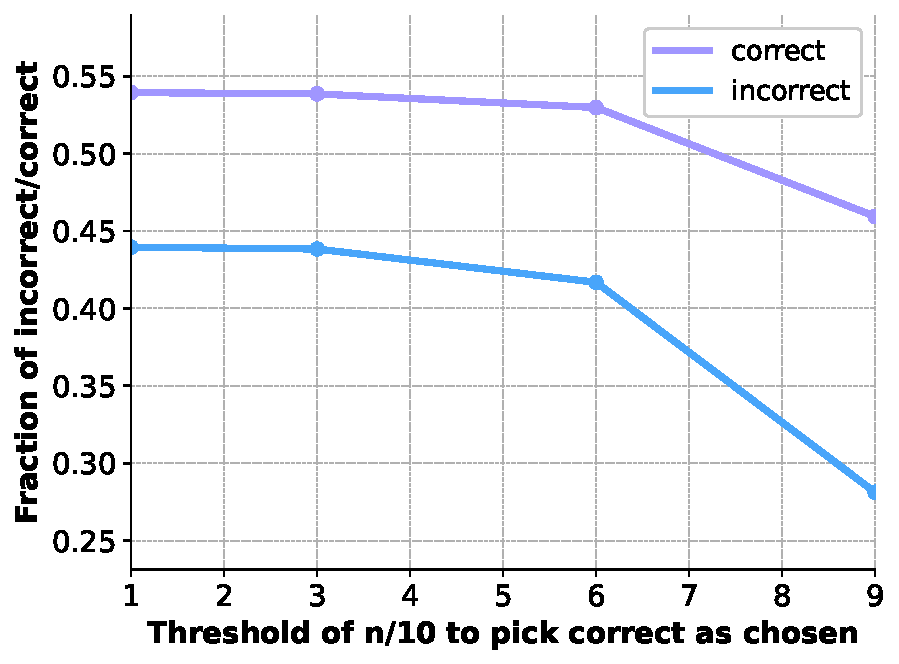
\includegraphics[width=0.75\linewidth]{posttraining/assets/dpo_factuality_ablations.pdf}
\caption{\label{fig:dpo_factuality_abaltions} DPO factuality ablations on LLama3 70b}
\end{figure}


Given the obvious degradation of performance in correctness in Figure \autoref{fig:dpo_factuality_abaltions} after 5/10, we take that value. This corresponds to roughly $4:4:10$ ratio of \textbf{trueVidk}:\textbf{trueVfalse}:\textbf{idkVfalse}
























\section{Posttraining: Results}
\label{appendix:posttraining_results}

In this section we report results for \llamathree posttrained models results on additional benchmarks and provide further benchmark details.


\subsection{Metric details and evaluation methodology}\label{appendix:posttraining_eval:methodology}

Details on metrics for each posttraining benchmark can be found in \autoref{tab:posttraining_benchmark_metric_details}.
\TODO{link to open source repo for evals}

\begin{table}
    \center
    \setlength{\tabcolsep}{3pt}
    \begin{tabular}{lrrl}
        \toprule
        \textbf{Benchmark} & \textbf{\# samples} & \textbf{\# few-shot} & \textbf{Metric} \\
        \midrule
        API-Bank~\citep{li2023api} & 391 & 0 & accuracy \\
        API-Bench~\citep{patil2023gorilla} & 1775 & 0 & accuracy \\
        ARC Challenge \citep{clark2018think} & 1165 & 0 & accuracy  \\
        BFCL~\citep{berkeley-function-calling-leaderboard} & 1700 & 0 & accuracy \\
        FActScore \citep{min2023factscore} & 500 & 0 & precision \\
        GPQA \citep{rein2023gpqagraduatelevelgoogleproofqa} & 448 & 0 & accuracy  \\
        GSM8K \citep{cobbe2021training} & 1319 & 8 & exact match  \\
        HumanEval \citep{chen2021evaluating} & 164 & 0 & pass@1  \\
        HumanEval+~\citep{liu2024your} & 164 & 0 & pass@1 \\
        IFEval \citep{zhou2023instruction} & 541 & 0 & prompt/instruction accuracy  \\
        InfiniteBench/En.QA \citep{zhang2024infty} & 351 & 0 & f1  \\
        InfiniteBench/En.MC \citep{zhang2024infty} & 229 & 0 & accuracy  \\
        MATH \citep{hendrycks2021measuring} & 5000 & 0/4 & sympy + judge  \\
        MBPP \citep{austin2021program} & 500 & 3 & pass@1 \\
        MBPP EvalPlus (base) \citep{liu2024your} & 378 & 0 & pass@1 \\
        MGSM \citep{shi2022languagemodelsmultilingualchainofthought} & 2750 & 8 & exact match  \\
        MMLU \citep{hendrycks2021mmlu} & 14042 & 0/5 & macro/micro accuracy  \\
        MMLU-Pro \citep{wang2024mmlu} & 12032 & 5 & macro/micro accuracy  \\
        MultiPL-E HumanEval ~\citep{cassano2022multiple} & 3025 & 0 & pass@1 \\
        MultiPL-E MBPP ~\citep{cassano2022multiple} & 7384 & 0 & pass@1  \\
        Needle-in-a-Haystack \citep{niah} & 225 & 0 & exact match  \\
        Nexus~\citep{srinivasan2023nexusraven} & 542 & 0 & accuracy \\
        ZeroSCROLLS/QuALITY \citep{zeroscrolls} & 21 & 0 & exact match  \\
        ZeroSCROLLS/Qasper \citep{zeroscrolls} & 28 & 0 & f1  \\
        ZeroSCROLLS/SQuALITY \citep{zeroscrolls} & 80 & 0 & rougeL  \\
        \bottomrule
    \end{tabular}
    \caption{\textbf{Few shot and metric settings for all posttraining benchmarks} used in the paper, in alphabetical order.
        \label{tab:posttraining_benchmark_metric_details}
    }
\end{table}






\subsection{Coding benchmarks: MultiPL-E results}\label{appendix:posttraining_results:coding}

We also observed significant improvements in performance of \llamathree in non-Python languages over post-training rounds, as displayed in \autoref{tab:multiple_MBPP_over_rounds}.




\begin{table}[t!]
\center
\setlength{\tabcolsep}{3pt}
\begin{tabular}{lrrr} %
\toprule
MultiPL-E & Round 4 & Round 5 & Round 6 \\
\midrule
HumanEval & 58.8\%  & 66.0\% & 69.25\% \\
MBPP  &  54.2\%  & 56.4\% & 60.8\% \\
\bottomrule
\end{tabular}%
\caption{\textbf{Improvement over rounds in MultiPL-E \citep{cassano2022multiple}}. We observed significant improvements in performance of \llamathree in non-Python languages in later rounds of posttraining primarily due to the inclusion of adding translated code data to our SFT mix.} \label{tab:multiple_MBPP_over_rounds}
\end{table}


\subsection{Multilingual benchmarks: Multilingual MMLU results}\label{appendix:mmlu_detailed_results}
We evaluate \llama3 models on multilingual MMLU. For each language, we report macro average accuracy across MMLU domains.
The \gpt metrics are taken from the technical paper. The \gpt4o metrics are gathered by running our evaluation pipeline and test set via OpenAI API.
Per-language results can be found in \autoref{tab:multilingual_mmlu_res}


  \begin{table}[t!]
      \center
      \setlength{\tabcolsep}{3pt}
      \begin{tabular}{lrrrrr}
      \toprule
          & \multicolumn{3}{c}{\llamathree}  & \\
          \cmidrule(lr){2-4}
          Language& 8B & 70B & 405B & \gpt (paper) & \gpto (API)\\
          \midrule

          Spanish & 62.4 & 80.0 & 85.1 & 84.0 & 86.7 \\
          Italian & 61.5 & 80.4 & 85.0 & 84.1 & 86.8 \\
          Portuguese & 62.1 & 80.1 & 85.0 & - & 86.9 \\
          French & 62.1 & 79.8 & 84.7 & 83.6 & 86.1 \\
          Romanian & 59.7 & 79.1 & 84.5 & - & 86.4 \\
          Dutch & 60.0 & 79.7 & 84.4 & - & 86.4 \\
          German & 60.3 & 79.3 & 84.4 & 83.7 & 86.0 \\
          Swedish & 58.8 & 79.2 & 83.9 & - & 86.7 \\
          Czech & 58.3 & 78.5 & 83.6 & - & 86.0 \\
          Indonesian & 58.3 & 79.2 & 83.6 & 83.1 & 85.7 \\
          Russian & 58.2 & 78.1 & 83.1 & 82.7 & 84.2 \\
          Polish & 56.4 & 77.6 & 82.8 & 82.1 & 85.2 \\
          Hungarian & 56.4 & 77.2 & 82.2 & - & 85.3 \\
          Chinese & 57.4 & 76.5 & 82.2 & - & 84.1 \\
          Greek & 53.0 & 77.0 & 82.1 & 81.4 & 85.6 \\
          Vietnamese & 56.0 & 76.5 & 81.5 & - & 83.5 \\
          Turkish & 53.7 & 76.1 & 80.8 & 80.0 & 84.0 \\
          Persian & 52.5 & 75.0 & 80.6 & - & 84.2 \\
          Japanese & 54.0 & 74.9 & 80.6 & 79.9 & 82.5 \\
          Hindi & 50.6 & 74.5 & 80.4 & - & 84.0 \\
          Finnish & 51.8 & 75.9 & 79.8 & - & 84.7 \\
          Korean & 51.7 & 73.2 & 79.1 & 77.0 & 81.9 \\
          Arabic & 50.8 & 74.1 & 78.9 & 80.0 & 83.6 \\
          Thai & 50.2 & 73.0 & 78.2 & 71.8 & 82.1 \\
          Bengali & 45.7 & 71.6 & 77.4 & 73.2 & 82.7 \\
          Telugu & 42.9 & 67.8 & 75.1 & 62.0 & 80.9 \\
          Swahili & 45.0 & 69.5 & 73.7 & 78.5 & 80.8 \\
          \bottomrule
      \end{tabular}
      \caption{\textbf{Multilingual MMLU}, an internal benchmark translated using Google Translate API. We evaluate our \llamathree models and \gpto with 5-shot, reporting macro average accuracy scores by language.  \label{tab:multilingual_mmlu_res}}
  \end{table}



\subsection{Multilingual benchmarks: FloRes200 results}\label{appendix:flores_detailed_results}

We analyzed our models on translation benchmarks to evaluate their content understanding and generation ability across multiple languages.
We used FloRes200 \citep{nllb2022} and report BLEU scores (spBLEU) for both translation directions (to/from English) and compare to GPT-4o and Seamless M4T v2\citep{communication2023seamlessmultilingualexpressivestreaming} in \autoref{tab:flores_res}. Per-language results can be found in \autoref{tab:flores_res_long_en_to_X} and \autoref{tab:flores_res_long_X_to_en}.

\begin{table}[t!]
  \center
   \setlength{\tabcolsep}{3pt}
  \begin{tabular}{lrrr} %
  \toprule

  Model& Size & English to X & X to English \\
  \midrule

  \multirow{ 2}{*}{\llamatwo}
  & 7B  & 6.9 & 11.9 \\
  &70B  & 17.7 & 23.1 \\
  \midrule

    \multirow{ 4}{*}{\llamathree}
    & 8B   & 27.1 & 36.1 \\
    & 70B  & 34.9 & 41.0 \\
    & 405B  & 37.4 & 43.6 \\
  \midrule

  \gpto & - & 38.6 & 42.5 \\
  SeamlessM4T v2 & - & 37.7 & 41.1 \\
  \bottomrule

  \end{tabular}
  \caption{\textbf{Flores200:} We report spBLEU scores for our \llamatwo and \llamathree family of models, in  both translation directions, averaged across 35 languages. We evaluate \gpto performance using the same method.
  \label{tab:flores_res}
  }
\end{table}


\begin{table}
  \center
   \setlength{\tabcolsep}{3pt}
  \begin{tabular}{lrrrr} %
  \toprule
 & \multicolumn{3}{c}{\llamathree}  & \\
        \cmidrule(lr){2-4}
  Target Language& 8B & 70B & 405B \\
  \midrule

    Portuguese & 48.1 & 53.0 & 54.9 \\
    French & 46.6 & 52.3 & 53.5 \\
    Swedish & 43.6 & 50.3 & 52.7 \\
    Indonesian & 39.3 & 45.3 & 47.6 \\
    German & 38.5 & 45.0 & 46.7 \\
    Romanian & 37.5 & 45.2 & 46.7 \\
    Vietnamese & 37.6 & 41.4 & 43.0 \\
    Czech & 31.0 & 37.6 & 41.0 \\
    Russian & 32.4 & 38.2 & 40.0 \\
    Turkish & 26.7 & 36.1 & 39.8 \\
    Thai & 28.4 & 36.5 & 39.5 \\
    Arabic & 25.7 & 35.9 & 38.9 \\
    Chinese (Simplified) & 30.2 & 35.9 & 38.3 \\
    Tagalog & 25.4 & 33.9 & 37.1 \\
    Hindi & 26.2 & 34.9 & 36.7 \\
    Italian & 31.6 & 34.5 & 36.7 \\
    Hungarian & 25.5 & 33.6 & 36.5 \\
    Greek & 25.7 & 33.1 & 36.4 \\
    Finnish & 22.6 & 32.3 & 35.7 \\
    Telugu & 20.6 & 32.2 & 35.7 \\
    Swahili & 17.8 & 30.6 & 35.5 \\
    Dutch & 29.9 & 34.6 & 35.3 \\
    Persian & 25.5 & 32.8 & 34.1 \\
    Malayalam & 16.8 & 29.8 & 33.8 \\
    Panjabi & 17.5 & 31.3 & 33.4 \\
    Bengali & 21.4 & 30.8 & 32.4 \\
    Spanish & 29.4 & 31.6 & 32.2 \\
    Kannada & 17.4 & 29.5 & 31.7 \\
    Polish & 25.2 & 29.7 & 31.3 \\
    Tamil & 17.1 & 28.3 & 31.0 \\
    Gujarati & 16.0 & 26.9 & 30.4 \\
    Japanese & 21.1 & 27.0 & 29.3 \\
    Urdu & 18.0 & 25.1 & 28.1 \\
    Korean & 19.3 & 25.0 & 27.7 \\
    Marathi & 13.7 & 23.0 & 25.7 \\
    \bottomrule
  \end{tabular}
  \caption{\textbf{FloRes200 (English to X)} spBLEU scores by language and \llamathree model sizes
  \label{tab:flores_res_long_en_to_X}
  }
\end{table}


\begin{table}[t!]
  \center
   \setlength{\tabcolsep}{3pt}
  \begin{tabular}{lrrrr} %
  \toprule
   & \multicolumn{3}{c}{\llamathree}  & \\
        \cmidrule(lr){2-4}
  Source Language& 8B & 70B & 405B \\
  \midrule
    Portuguese & 51.0 & 54.2 & 56.1 \\
    French & 46.1 & 49.9 & 52.6 \\
    Swedish & 48.4 & 51.7 & 54.9 \\
    Indonesian & 43.6 & 47.4 & 51.0 \\
    German & 45.5 & 49.9 & 51.9 \\
    Romanian & 43.9 & 47.8 & 50.5 \\
    Vietnamese & 36.5 & 40.2 & 42.9 \\
    Czech & 41.9 & 45.3 & 48.1 \\
    Russian & 38.6 & 42.0 & 43.1 \\
    Turkish & 36.7 & 42.5 & 45.1 \\
    Thai & 32.1 & 35.3 & 38.4 \\
    Arabic & 39.4 & 45.5 & 48.3 \\
    Chinese (Simplified) & 30.6 & 33.9 & 36.6 \\
    Tagalog & 40.3 & 48.0 & 51.2 \\
    Hindi & 38.9 & 44.3 & 46.8 \\
    Italian & 35.7 & 38.7 & 39.9 \\
    Hungarian & 35.7 & 40.0 & 42.4 \\
    Greek & 35.6 & 40.3 & 42.6 \\
    Finnish & 34.2 & 39.1 & 41.8 \\
    Telugu & 33.5 & 38.9 & 42.2 \\
    Swahili & 33.1 & 43.2 & 46.6 \\
    Dutch & 33.8 & 37.1 & 38.2 \\
    Persian & 36.6 & 40.8 & 43.3 \\
    Malayalam & 31.2 & 37.3 & 39.6 \\
    Panjabi & 32.1 & 40.3 & 43.5 \\
    Bengali & 31.6 & 38.1 & 40.7 \\
    Spanish & 32.9 & 35.2 & 36.4 \\
    Kannada & 29.4 & 35.2 & 37.8 \\
    Polish & 32.0 & 35.7 & 37.7 \\
    Tamil & 28.1 & 35.3 & 37.1 \\
    Gujarati & 32.7 & 38.2 & 42.7 \\
    Japanese & 28.6 & 32.7 & 35.1 \\
    Urdu & 31.5 & 38.8 & 41.4 \\
    Korean & 31.2 & 33.7 & 37.5 \\
    Marathi & 31.6 & 39.0 & 41.1 \\
        \bottomrule

  \end{tabular}
  \caption{\textbf{FloRes200 (English to X)} spBLEU scores by language and \llamathree model sizes
  \label{tab:flores_res_long_X_to_en}
  }
\end{table}


\subsection{Zero-shot Tool Use Evaluation}\label{appendix:tools_benchmarks}

We evaluate our models on the following function calling benchmarks:
\begin{itemize}
    \item \textbf{Nexus} evaluates the an LLM's ability of doing \textit{single, parallel, and nested function calls in single-turn dialogues}. The model takes as input a natural language instruction, along with the function definition and docstring for all available function calls, and output appropriate function calls. Each test sample contains multiple candidate functions: the ground truth one and other similar functions that are not needed for solving the user query, thereby making it more challenging for the model to select the correct function. The model output is evaluated by comparing it with the ground truth by executing the function call and ensuring the arguments match the ground truth exactly. The examples are inspired by real-world use cases such as comparing reviews, retrieving comments from a website, finding the distance between two venues, or finding the cheapest hotels in a given city. While current state-of-the-art LLMs are reasonably good at single funcion calls, they still struggle with parallel and nested function calls which are common in real-world applications. Hence, Nexus provides a good function calling testbed and is far from being saturated, with the best models solving only $50-60\%$ of the queries. The benchmark contains two domains: a generic one and a cybersecurity one. The generic domain contains two popular benchmarks in the literature, namely the ToolAlpacaSimulated~\citep{tang2306toolalpaca} dataset and the ToolLLM~\citep{qin2023toolllm} dataset, which were generated by GPT-3.5 and filetered for correctness. The cybersecurity subset of the benchmark consists of human queries for operating CVE and CPE Search, VirusTotal V3, and EmailRep where the ground truth answers were verified by cybersecurity experts. The examples are inspired by real-world use cases, making this a realistic benchmark.

    \item \textbf{API-Bank} evaluates an LLM's ability of performing function calls in a \textit{multiturn dialogue} that may include other function calls from either the user or the assistant. In contrast with Nexus, this benchmark focuses on multi-turn dialogues and single function calls, although a small fraction of the test samples require nested function calls. It consists of 391 tool-use dialogues with 753 API calls in total from a set of 73 APIs resembling tools found in the real-world. The examples are inspired from real-world scenarios such as changing a user's password, opening a bank account, scheduling meetings, or modifying appointments. The model often needs to extract more information from the user before solving the task, such as the user's password or scheduling preferences. API-Bank is not as challenging as Nexus for state-of-the-art LLMs, with most of them achieving $\textgreater 85\%$ success rate.

    \item \textbf{Gorilla API-Bench} evaluates an LLM's ability of selecting from a \textit{large, overlapping, and changing set of tools} expressed using their APIs and API documentation. API-Bench was created by scraping \textit{machine learning model APIs} from three public hubs, namely TorchHub (94 APIs), TensorHub (696 APIs), and HuggingFace (925 APIs based on the most downloaded 20 models per task category). The model APIs cover a wide range of domains such as multimodal, computer vision, natural language processing, audio, tabular data, and reinforcement learning. For each API, 10 synthetic user questions are generated using self-instruct~\cite{wang2023selfinstructaligninglanguagemodels}. API-Bench uses a common AST sub-tree matching technique to evaluate the functional correctness of the generated API. We consider the zero-shot evaluation mode presented in the original paper rather than the retriever-based one. This benchmark is also quite challenging for current state-of-the-art models with most of them achieving around $30-40\%$ success rate.

    \item \textbf{Berkeley Function Calling Leaderboard (BFCL)} evaluates an LLM's ability of using APIs to assist with user queries. The leaderboard consists of real-world data and is updated periodically. For more information on the evaluation dataset and methodology, please refer to our blog post and code release. This benchmark consists of 2000 question-function-answer pairs from \textit{multiple coding languages} (i.e. 100 Java, 50 JavaScript, 70 REST API, 100 SQL, and 1,680 Python), \textit{diverse application domains} (e.g., computing, cloud, sports, or law), and a \textit{wide range of scenarios} (simple where a single API is provided and the model needs to use this API with the correct arguments, multiple where multiple APIs are provided and the model has to select which one to use and with what arguments, parallel where only one API is provided and the model needs to invoke multiple function calls in parallel, and parallel multiple where multiple APIs are provided and the model needs to make invoke multiple function calls). BFCL also tests the LLMs' ability of not performing any function calls when none of the available functions are relevant for the user's query. The model answers are evaluated using both AST and execution. This benchmark turns out to be easier than API-Bench or Nexus for top LLMs with most of them solving $\textgreater 85\%$ queriess.
\end{itemize}


For Nexus, API-Bench, and BFCL, we use their corresponding open-source implementations for the evaluation function and prompt. In the case of API-Bank, we discovered inaccuracies in the benchmark that led to false negatives when evaluating LLMs. To address this issue, we make two major improvements to the existing benchmark. First, we correct and complete ground truth answers that were initially incorrect or incomplete (i.e. they did not contain all valid solutions). Second, we enhance the evaluation metric to better capture the function call correctness. Certain keyword arguments have a unique ground truth value while others accept any string with the same semantic meaning as the reference value. Hence, we split keyword arguments into two groups and use exact match for the former and ROUGE score for the latter. We also use a more detailed zero-shot prompt, \textit{e.g.}, asking \llamathree to avoid proposing calls that are already executed in the dialog:
\begin{framed}
You are given multiple functions, and a user query or a dialog between a user and an AI.

        In both cases, please proceed with generating a function call for the appropriate function with the proper arguments that best answers the given case.

        Don't re-do calls that were already executed in the dialog: just use their output in your call.

        Respond with nothing but the function call ONLY, such that I can directly execute your function call without any post processing necessary from my end.
        Don't forget to include the keywords of the function's arguments in your call. Do not include arguments that have a default and that you don't need to modify.
        Do not use intermediate variables.

        \{\{ tools \}\}

        User query or dialog:

        \{\{ additional\_info \}\}

        Question: \{\{ question \}\}
\end{framed}

We open-source our revised implementation of API-Bank and encourage the community to use it for more accurate evaluation.


\subsection{Human Evaluation on Tool Use}
\label{appendix:tools_human_evals}

As mentioned in ~\ref{subsection:human_evals_tool_use}, we conducted pairwise evaluations with human annotators to evaluate the tool use capabilities of \llamathree versus \gpt4o and \gptfourturbo. This section details the prompt collection process, guidelines for human annotators and improvement of the tool use capabilities of the model with the post-training rounds.
\subsubsection{Prompt Collection}
Here we provide more details on the set of prompts used to run human evaluations for tool use. We collect prompts from the following sources:
\begin{itemize}
    \item LMSys dataset~\citep{chiang2024chatbot}: We select 1500 prompts from the LMSys public datasets, keeping only the prompts that require code execution and API calling (including plotting and file uploads). We then use \llamathree 405B and \gpt4o to remove prompts which were unclear or not relevant. Some prompt examples are “debug and run the following compressing png python code.” or “Generate the 15th Fibonacci number.”

    \item GAIA benchmark~\citep{mialon2023gaia}: We select 93 prompts related to file uploads from GAIA, which involve files supported by the model, such as \textsc{.xlsx, .csv, .py, .pdf, .docx, .txt, .png, .jpg}. Some examples are “The attached Excel file contains the sales of menu items for a local fast-food chain. What were the total sales that the chain made from food (not including drinks)?”

    \item Human annotators: We collect 150 samples from human annotators, who were asked to generate prompts based on specific guidelines to test the model’s ability of solving tasks based on a file uploaded by the user such as content summarization, question answering, data analysis or visualization. For example, “Given the provided CSV file containing sports data, generate a bar chart showing the distribution of goals scored by each player.”

    \item Synthetic generation: We also generate 600 prompts related to code execution and plot generation using \gpt4o, \sonnet, \llamathree and Gemini 1.5 Pro. Some examples include “Calculate the factorial of 15 using a recursive function.”. The generated prompts were then verified, de-duplicated, and cleaned manually. The prompt used to generate these queries was a variation of “Show me some queries which can test code execution for an LLM. Make sure there are specific examples which this can be tested on.”

\end{itemize}

\subsubsection{Guidelines for Human Annotators}
Human annotators who are skilled in Python coding and fluent in English language are selected to rate the two responses from different models given a prompt. We gather three annotations per prompt and aggregate the results to get a response.

Here we use a 5-point scale for human ratings, where the scale is defined as follows: (1) Response A is significantly better, (2) Response A is slightly better (3) Both responses are about equally good, (4) Response B is slightly better, (5) Response B is significantly better.

Annotators are also asked to provide an explanation for their rating and categorize the issues with the response, if any, among the following categories:
\begin{itemize}
\item Accuracy issues: Incorrect code or response, lack of logic, hallucination
\item Relevance issues: Off-topic response
\item Completeness issues: Failure to address an important aspect of the prompt or request, not offering the necessary explanation when it's expected, missing labels in plots
\item Fluency issues: Coherence issues
\item Formatting issues: Unclear formatting,  unaesthetic plots
\end{itemize}

The breakdown of the issues for \llamathree by category as annotated by the human labelers is shown in ~\cref{fig:heval-tools-issues}.

\begin{figure}
\centering
\begin{subfigure}{.4\textwidth}
  \centering
  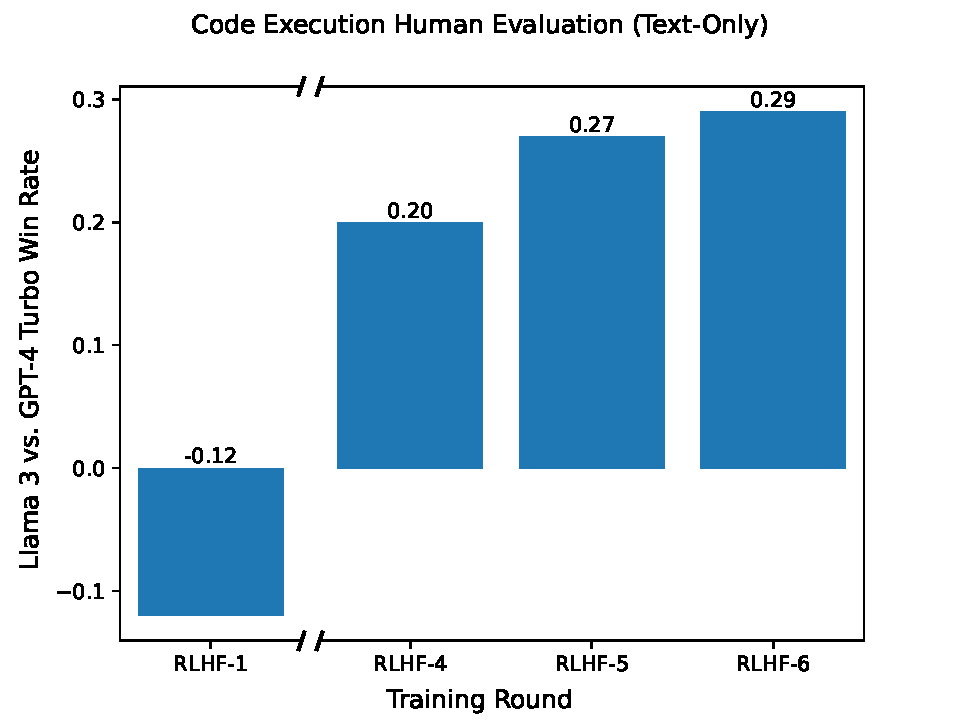
\includegraphics[width=\linewidth]{{assets/tool_human_evals_history.pdf}}
  \caption{Win Rate of \llamathree vs \gptfourturbo}
  \label{fig:heval-tools-history}
\end{subfigure}%
\begin{subfigure}{.4\textwidth}
  \centering
  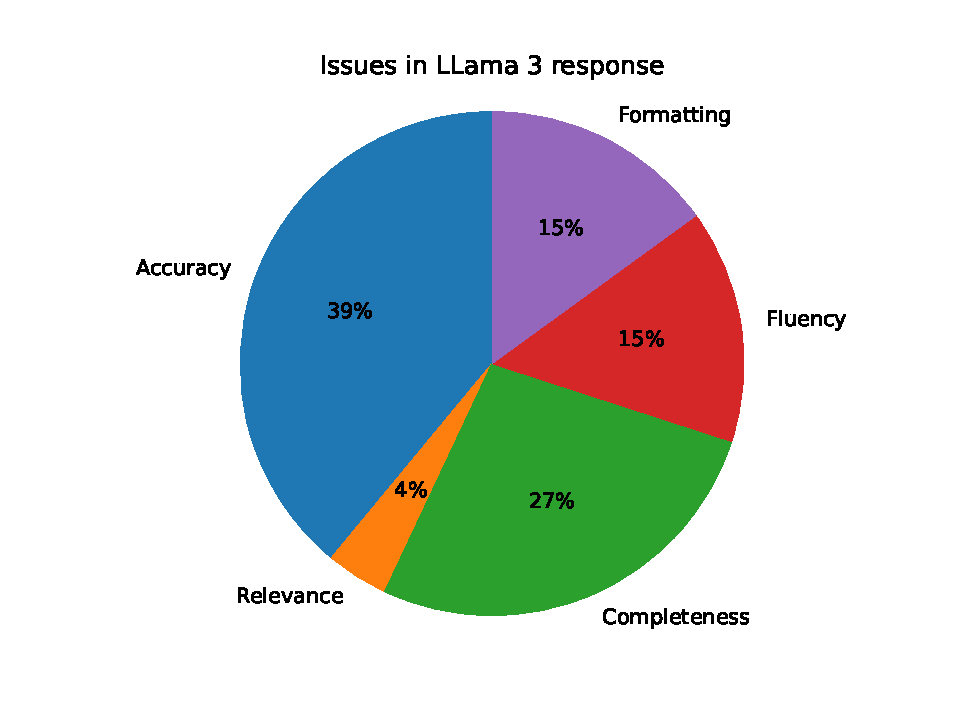
\includegraphics[width=\linewidth]{{assets/tool_human_evals_issues.pdf}}
  \caption{Issues in \llamathree responses}
  \label{fig:heval-tools-issues}
\end{subfigure}
\caption{(a)  \llamathree steadily improves relative to \gptfourturbo on code execution (without plotting or file uploads) throughout multiple post-training rounds (b) breakdown of the issues for \llamathree by category as annotated by the human labelers. }
\label{fig:heval-tools-history-issues}
\end{figure}

\subsubsection{Model Improvement with Post-Training Rounds}

As~\cref{fig:heval-tools-history} shows, \llamathree steadily improves relative to \gptfourturbo on code execution (without plotting or file uploads) throughout multiple finetuning rounds. The net win rate of \llamathree after the first post-training round versus \gptfourturbo (version: gpt-4-turbo-2024-04-09) was 38\% with a 12\% neutral rate, but went up to 54\% with a 20\% neutral rate in the final round after five stages of post-training.




\subsection{Factuality benchmarks: FActScore results}
\paragraph{Factuality}






We report results on FActScore \citep{min2023factscore} to measure the model's performance in factuality. Since on of the openai models defined for FActScore \cite{min2023factscore} have been deprecated, we replaced the chosen models with their recommended replacements as defined by openai, switching 'text-davinci-003' for 'gpt-3.5-turbo-instruct', see \cite{openai2024deprecations}.
We prompt each model asking for biographies on the 500 entities in the same manner as defined in \cite{min2023factscore}. Results are shown in \autoref{tab:factuality_metrics}.

\begin{table}[t!]
  \begin{NiceTabular}{lcc}
	\CodeBefore
	\Body
	\toprule
&FActScore & \textit{Winrate}\\
\cmidrule{2-2}
	Llama 3 8B & \textbf{62.1 \scriptsize{$\pm$4.3}} & \textit{1}\\
	Gemma 9B - it &\textbf{67.9 \scriptsize{$\pm$4.1}} & \textit{1}\\
	Mistral 7B Instruct &48.7 \scriptsize{$\pm$4.4} & \textit{0}\\
	\midrule
	Llama 3 70B & \textbf{74.1 \scriptsize{$\pm$3.8}} & \textit{1}\\
	Mixtral-8x22B Instruct &\textbf{69.9 \scriptsize{$\pm$4.0}} & \textit{1}\\
	GPT-3.5 Turbo &\textbf{76.1 \scriptsize{$\pm$3.7}} & \textit{1}\\
	\midrule
	Llama 3 405B & 77.0 \scriptsize{$\pm$3.7} & \textit{0}\\
	GPT-4 (0125) &\textbf{87.9 \scriptsize{$\pm$2.9}} & \textit{1}\\
	GPT-4 Omni &\textbf{88.3 \scriptsize{$\pm$2.8}} & \textit{1}\\
	Claude-3.5 Sonnet &80.0 \scriptsize{$\pm$3.5} & \textit{0}\\
	Nemotron &70.1 \scriptsize{$\pm$4.0} & \textit{0}\\
	\bottomrule
\end{NiceTabular}

  \caption{\textbf{FActScore results.} We report results on FActScore \citep{min2023factscore}.}
  \label{tab:factuality_metrics}
\end{table}



\subsection{Human Evaluation: Taxonomy}
\label{section:taxonomy_human_eval}

To ensure comprehensiveness of the prompt sets in human evaluations,
we built taxonomy with categories and subcategories.
More concretely,
Table~\ref{table:taxonomy_english_multilingual}--\ref{table:taxonomy_coding}
and Table~\ref{table:taxonomy_multi_turn_english}--\ref{table:taxonomy_multi_turn_coding}
present
the taxonomy for individual capabilities (English, multilingual, reasoning, and coding)
and multiturn capabilities (English, reasoning, and coding), respectively.

\begin{table*}[t]
    \centering
    \begin{NiceTabular}{ll}
    \CodeBefore
    \rectanglecolor{metabg}{2-1}{100-1}
    \Body
    \toprule

                               Categories & Subcategories             \\
    \midrule
\multirow{5}{*}{Factual Questions}	& Historical events \& figures \\
	& Scientific concepts and explanations \\
	& Geographical information \\
	& Cultural \& social topics \\
	& Technical information \\


\midrule
	\multirow{8}{*}{Procedural Questions}	& Cooking \& food preparation \\
	& Home \& DIY projects \\
	& Technology \& devices \\
	& Arts \& crafts \\
	& Travel \& transportation \\
	& Finance \& budgeting \\
	& Work \& productivity \\
	& Health \& fitness \\


\midrule
	\multirow{1}{*}{Language assistance}	& Grammar, spelling, \& vocabulary \\


\midrule
	\multirow{9}{*}{Writing \& content creation}	& Analysis \\
	& Creative writing:  Fiction \\
	& Creative writing:  Poetry and Songwriting \\
	& Creative writing: Social media posts \\
	& Creative writing: Nonfiction \\
	& Business writing \\
	& Legal writing \\
	& Classification \\
	& Summarization \& editing \\



\midrule
	\multirow{6}{*}{Dialogue}	& Identity / Personas \\
	& Chit-Chat \\
	& Advice \\
	& Games: Choose-your-own-adventure \\
	& Games: Word \& language \\
	& Games: Social \& party \\


\midrule
	\multirow{4}{*}{Recommendations / Brainstorming}	& Dining \& food suggestions \\
	& Entertainment suggestions \\
	& Travel \& destinations suggestions \\
	& Product \& service recommendations \\


\midrule
	\multirow{8}{*}{Personal Growth and Development}	& Build confidence and self-esteem \\
	& Emotional support \\
	& Goal setting \\
	& Motivation \\
	& Physical health support \\
	& Professional and career support \\
	& Relationship support \\
	& Tutoring and learning support \\



\midrule
	\multirow{4}{*}{Social interaction and communication}	& Debate and opinions \\
	& Discuss shared interests \\
	& Humor and jokes \\
	& Socialize with friends (group chat) \\

    \bottomrule
    \end{NiceTabular}
    \caption{Taxonomy of the English and multilingual capabilities.}
    \label{table:taxonomy_english_multilingual}
\end{table*}












\begin{table*}[t]
\centering
\begin{NiceTabular}{ll}
\CodeBefore
\rectanglecolor{metabg}{2-1}{100-1}
\Body
\toprule
Categories & Subcategories             \\

\midrule
\multirow{15}{*}{Mathematical Calculation} & Arithmetic \& basic math \\
& Algebra \& equations \\
& Geometry \& trigonometry \\
& Calculus \& advanced math \\
& Probability \& statistics \\
& Discrete math \& logic \\
& Ordinary and partial differential equations \\
& Math word problem solving \\
& Math question answering \\
& Theorem proving (e.g., proofs) \\
& Mathematical model building \\
& Physical reasoning \\
& Temporal reasoning \\
& Spatial reasoning \\
& Identifying root causes \& issues \\
& Evaluating evidence \& reasoning \\

\midrule
\multirow{7}{*}{Commonsense Reasoning} & Identifying pros \& cons \\
& Inductive reasoning \\
& Deductive reasoning \\
& Empathy and perspective taking \\
& Social norm understanding \\
& Humor understanding \\
& Negotiation \\

\midrule
\multirow{8}{*}{Logic / problem solving} & Emotion recognition / sentiment analysis \\
& Consequence evaluation \\
& Applying moral and ethical principles \\
& Resolving moral or ethical dilemmas (conflict of principles) \\
& Hypothesis formation and testing \\
& Causal reasoning \\
& Scientific evidence evaluation \\
& Model-based reasoning \\

\midrule
\multirow{6}{*}{Social and Emotional Reasoning} & Case-Based Reasoning \\
& Statutory Interpretation \\
& Contract Interpretation \\
& Administrative Regulation Interpretation \\
& Legal Evidence Evaluation \\
& Moral and Ethical Reasoning \\

\midrule
\multirow{2}{*}{Scientific Reasoning} & Applying moral and ethical principles \\
& Resolving moral or ethical dilemmas (conflict of principles) \\

\bottomrule
\end{NiceTabular}
\caption{Taxonomy of the reasoning capability.}
\label{table:taxonomy_reasoning}
\end{table*}



\begin{table*}[t]
\centering
\begin{NiceTabular}{ll}
\CodeBefore
\rectanglecolor{metabg}{2-1}{100-1}
\Body
\toprule
Categories & Subcategories             \\

\midrule
\multirow{5}{*}{Code generation / synthesis} & Code generation (Text to Code) \\
& Code completion \\
& Code Summarization / Compression \\
& Code to Code (same language) \\
& CLI \\

\midrule
\multirow{5}{*}{Code documentation} & Comment generation \\
& Commit text generation \\
& Document this function \\
& Create example usages of this function \\
& Create API documentation \\
\midrule
\multirow{2}{*}{Code debugging} & Debugging \& troubleshooting \\
& Testing \\
\midrule
\multirow{4}{*}{Code review \& Code review} & Code review \\
& Security Review \\
& Quality Assurance \\
& Log Analysis (Text to Text) \\
\bottomrule
\end{NiceTabular}
\caption{Taxonomy of the coding capability.}
\label{table:taxonomy_coding}
\end{table*}
















\begin{table*}[t]
    \centering
    \begin{NiceTabular}{ll}
    \CodeBefore
    \rectanglecolor{metabg}{2-1}{100-1}
    \Body
    \toprule
Categories & Subcategories             \\

\midrule
	\multirow{6}{*}{Dialogue}	& Identity / Personas \\
	& Chit-Chat \\
	& Advice \\
	& Games: Choose-your-own-adventure \\
	& Games: Word \& language \\
	& Games: Social \& party \\


\midrule
	\multirow{4}{*}{Recommendations / Brainstorming}	& Dining \& food suggestions \\
	& Entertainment suggestions \\
	& Travel \& destinations suggestions \\
	& Product \& service recommendations \\


\midrule
	\multirow{8}{*}{Personal Growth and Development}	& Build confidence and self-esteem \\
	& Emotional support \\
	& Goal setting \\
	& Motivation \\
	& Physical health support \\
	& Professional and career support \\
	& Relationship support \\
	& Tutoring and learning support \\



\midrule
	\multirow{4}{*}{Social interaction and communication}	& Debate and opinions \\
	& Discuss shared interests \\
	& Humor and jokes \\
	& Socialize with friends (group chat) \\

    \bottomrule
    \end{NiceTabular}
    \caption{Taxonomy of the multiturn English capability.}
    \label{table:taxonomy_multi_turn_english}
\end{table*}



\begin{table*}[t]
    \centering
    \begin{NiceTabular}{ll}
    \CodeBefore
    \rectanglecolor{metabg}{2-1}{100-1}
    \Body
    \toprule
Categories & Subcategories             \\

\midrule
\multirow{4}{*}{Mathematical Reasoning}

& Math word problem solving \\
& Math question answering \\
& Theorem proving (e.g., proofs) \\
& Mathematical model building \\

\midrule
\multirow{3}{*}{Commonsense Reasoning}
& Physical reasoning \\
& Temporal reasoning \\
& Spatial reasoning \\
\midrule

\multirow{5}{*}{Logic /problem solving}
& Identifying root causes \& issues \\
& Evaluating evidence \& reasoning \\
& Identifying pros \& cons \\
& Inductive reasoning \\
& Deductive reasoning \\

\midrule
\multirow{4}{*}{Social and Emotional Reasoning}
& Empathy and perspective taking \\
& Social norm understanding \\
& Emotion recognition / sentiment analysis \\

\midrule
\multirow{3}{*}{Moral and Ethical Reasoning}
& Consequence evaluation \\
& Applying moral and ethical principles \\
& Resolving moral or ethical dilemmas (conflict of principles) \\

\midrule
\multirow{3}{*}{Scientific Reasoning}
& Hypothesis formation and testing \\
& Causal reasoning \\
& Model-based reasoning \\

    \bottomrule
    \end{NiceTabular}
    \caption{Taxonomy of the multiturn reasoning capability.}
    \label{table:taxonomy_multi_turn_reasoning}
\end{table*}


\begin{table*}[t]
    \centering
    \begin{NiceTabular}{ll}
    \CodeBefore
    \rectanglecolor{metabg}{2-1}{100-1}
    \Body
    \toprule
Categories & Subcategories             \\

\midrule
\multirow{2}{*}{Code explanation} & Code walkthroughs \\
& Algorithm explanations \\
\midrule

\multirow{2}{*}{Code debugging}
& Debugging \& troubleshooting \\
& Testing \\

\midrule
\multirow{5}{*}{Programming Assistant}
& Code Understanding \\
& Problem decomposition \\
& Algorithmic reasoning \\
& Debugging reasoning \\
& Code optimization \\

\midrule
\multirow{6}{*}{Chat Model}

& Code generation / synthesis \\
& Code documentation \\
& Code debugging \\
& Code review \& Best practices \\
& Coding Q\&A (text -> text) \\
& Code explanation \\


    \bottomrule
    \end{NiceTabular}
    \caption{Taxonomy of the multiturn coding capability.}
    \label{table:taxonomy_multi_turn_coding}
\end{table*}







\subsection{Human Evaluation: Difficulty of Prompts}
\label{section:difficulty_human_eval}

To illustrate difficulty of prompts in human evaluations (Section~\ref{section:human_evals}), below is a summary of the definitions, accompanied by examples, for easy, medium, and hard levels for the English and multilingual capabilities. Note that the following examples are for illustrations only, and they are not from the human evaluation prompt set.

\subsubsection{Easy}

\paragraph{Definition} Prompt is a single ask/requirement/constraint for the model presented as a single statement OR prompt is a single statement without ask/requirement/constraints AND would not require subject matter expertise to understand.

\paragraph{Examples}

\begin{itemize}
    \item Illustrate and explain the proper use of a semi-colon.
    \item How do I uninvite my brother to my wedding?
    \item I've been having trouble sticking to my healthy diet lately. Give me some motivational words or tips to help me make better food choices and achieve my health goals.
\end{itemize}

\subsubsection{Medium}

\paragraph{Definition} Prompt includes 2--4 asks/requirements/constraints for the model AND would not require subject matter expertise to produce a response.

\paragraph{Examples}

\begin{itemize}
    \item My neighbors blast loud music all night, and I can’t sleep. I’ve tried talking to them directly, as well as calling 311 but nothing has changed. What else do you think I can try?
    \item How do I ask my boss for a raise? I think I’m underpaid but my boss never has time for me.
    \item Pretend you’re Bugs Bunny. I’m Elmer Fudd. How would you greet me?
    \item Write me a funny haiku about dogs.
\end{itemize}

\subsubsection{Hard}

\paragraph{Definition} Prompt contains 5 or more asks/requirements/constraints for the model OR requires subject matter expertise above and beyond “common knowledge” in order to respond.

\paragraph{Examples}

\begin{itemize}
    \item Write a poem to say sorry to my dog because I didn't spend enough time with it. The poem should have 26 lines where each line begins with Z, Y, X, ..., A, respectively, and always ends with h. The poem cannot contain any animal words.
    \item Sort the following words alphabetically, and in the result remove the first and the fourth words while capitalize the rest: sioux fortescue purloin percept helmsman friend friends. Append a new lower-case word that is an animal living in Antarctica. Output the result with numbered bullets.
    \item Handling long-sequence inputs presents a significant challenge to the KV-cache of Transformers.  Can we address this challenge better by training Transformers with more GPUs?
    \item I’m hosting a dinner party next week. I have a kosher friend coming, but also a vegan friend. Also, I am allergic to nuts. My husband likes spicy food. There might be a few picky eaters who are coming too. They may come with kids who attend preschools. What do you think I should make for dinner? And what about drinks?
\end{itemize}


\subsection{Human Evaluation: Detailed Results}
\label{section:detailed_human_eval}

Figure~\ref{fig:heval-gpt4o-difficulty} shows human evaluation results for Llama 3 405B vs. GPT-4 (0125 API version) across varying difficulty levels (Appendix~\ref{section:difficulty_human_eval}). Figure~\ref{fig:heval-gpt4o-english-l1.png}--\ref{fig:heval-gpt4o-portuguese-l2.png}  compare the individual capabilities (English, reasoning, and coding, Hindi, Spanish, and Portuguese) of Llama 3 405B vs. GPT-4 (0125 API version) across categories and subcategories (Appendix~\ref{section:taxonomy_human_eval}).
Finally, Figure~\ref{fig:heval-gpt4o-multiturn-english-l1.png}--\ref{fig:heval-gpt4o-multiturn-coding-l2.png} assess their multiturn capabilities in English, reasoning, and coding.






\begin{figure}
    \centering
    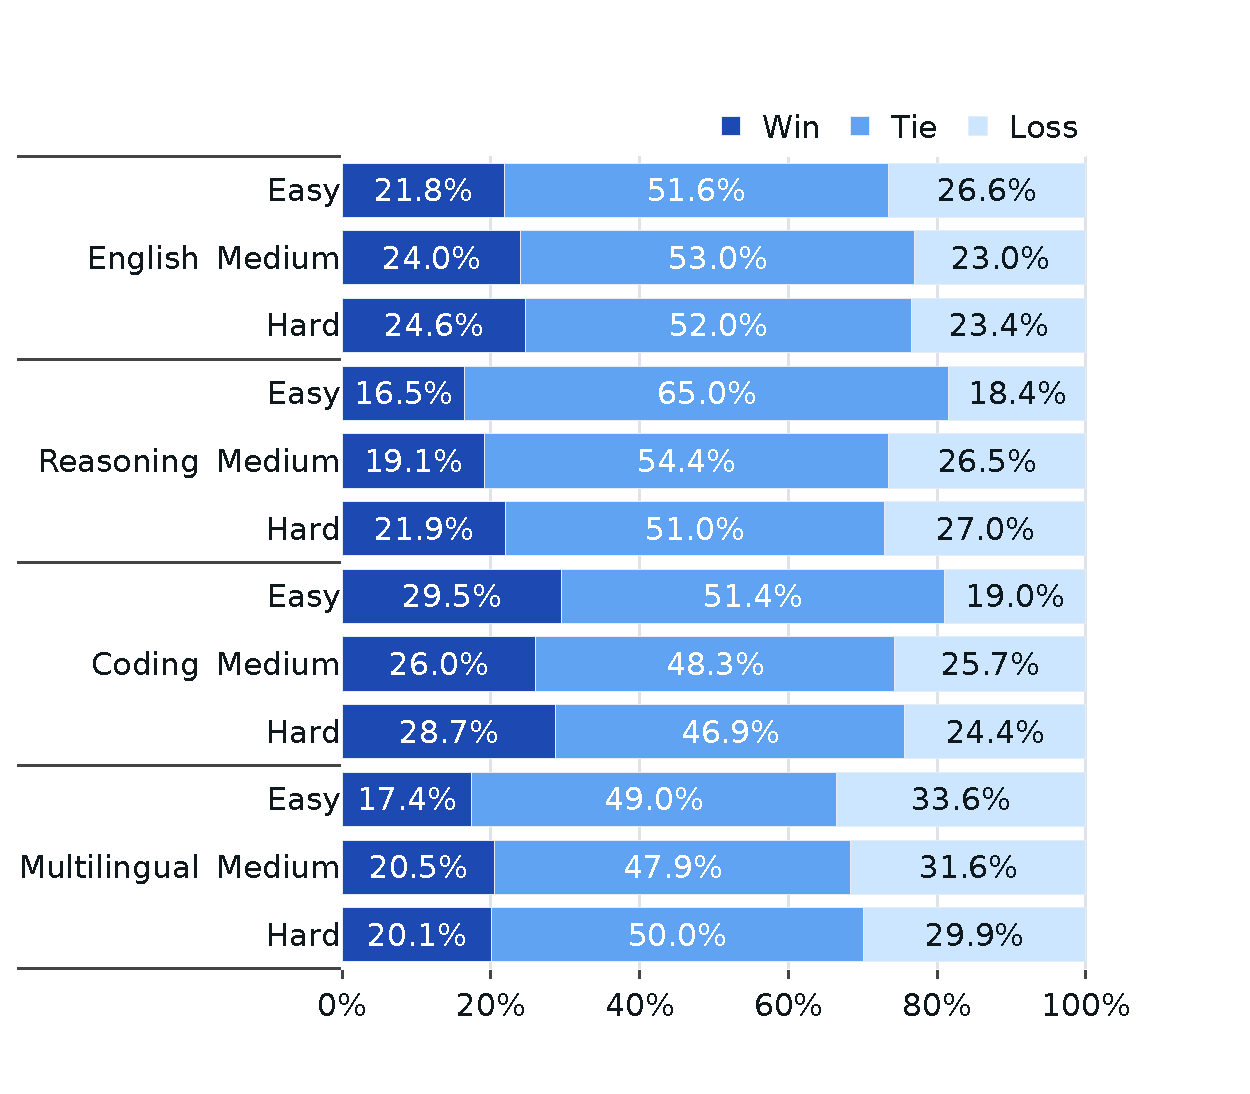
\includegraphics[width=0.75\linewidth]{assets/heval-gpt4preview-difficulty.pdf}
    \caption{Human evaluation results for Llama 3 405B vs. GPT-4 across varying difficulty levels.}
    \label{fig:heval-gpt4o-difficulty}
\end{figure}


\begin{figure}
    \centering
    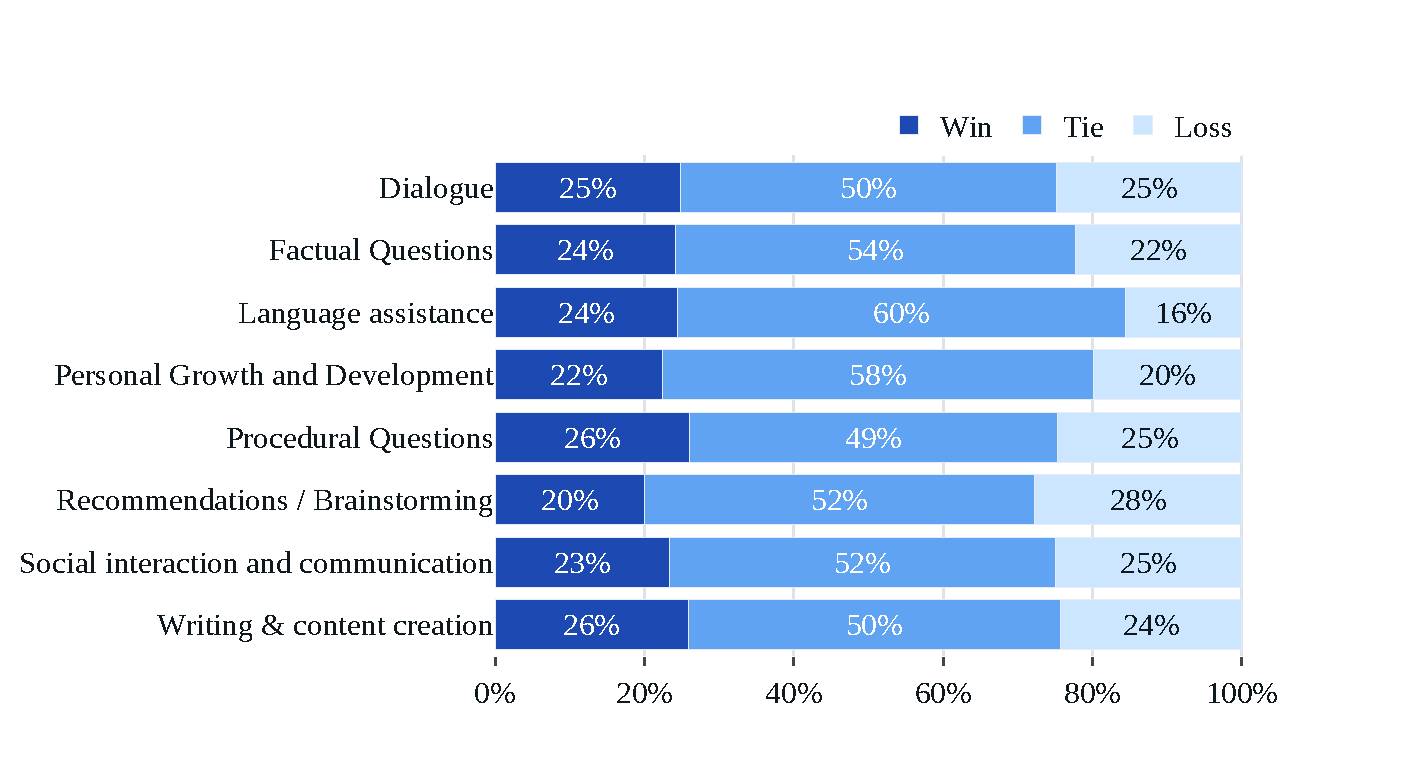
\includegraphics[width=0.75\linewidth]{assets/heval-gpt4preview-english-l1.pdf}
    \caption{Human evaluation results comparing the English capability of Llama 3 405B vs. GPT-4 across categories.}
    \label{fig:heval-gpt4o-english-l1.png}
\end{figure}


\begin{figure}
    \centering
    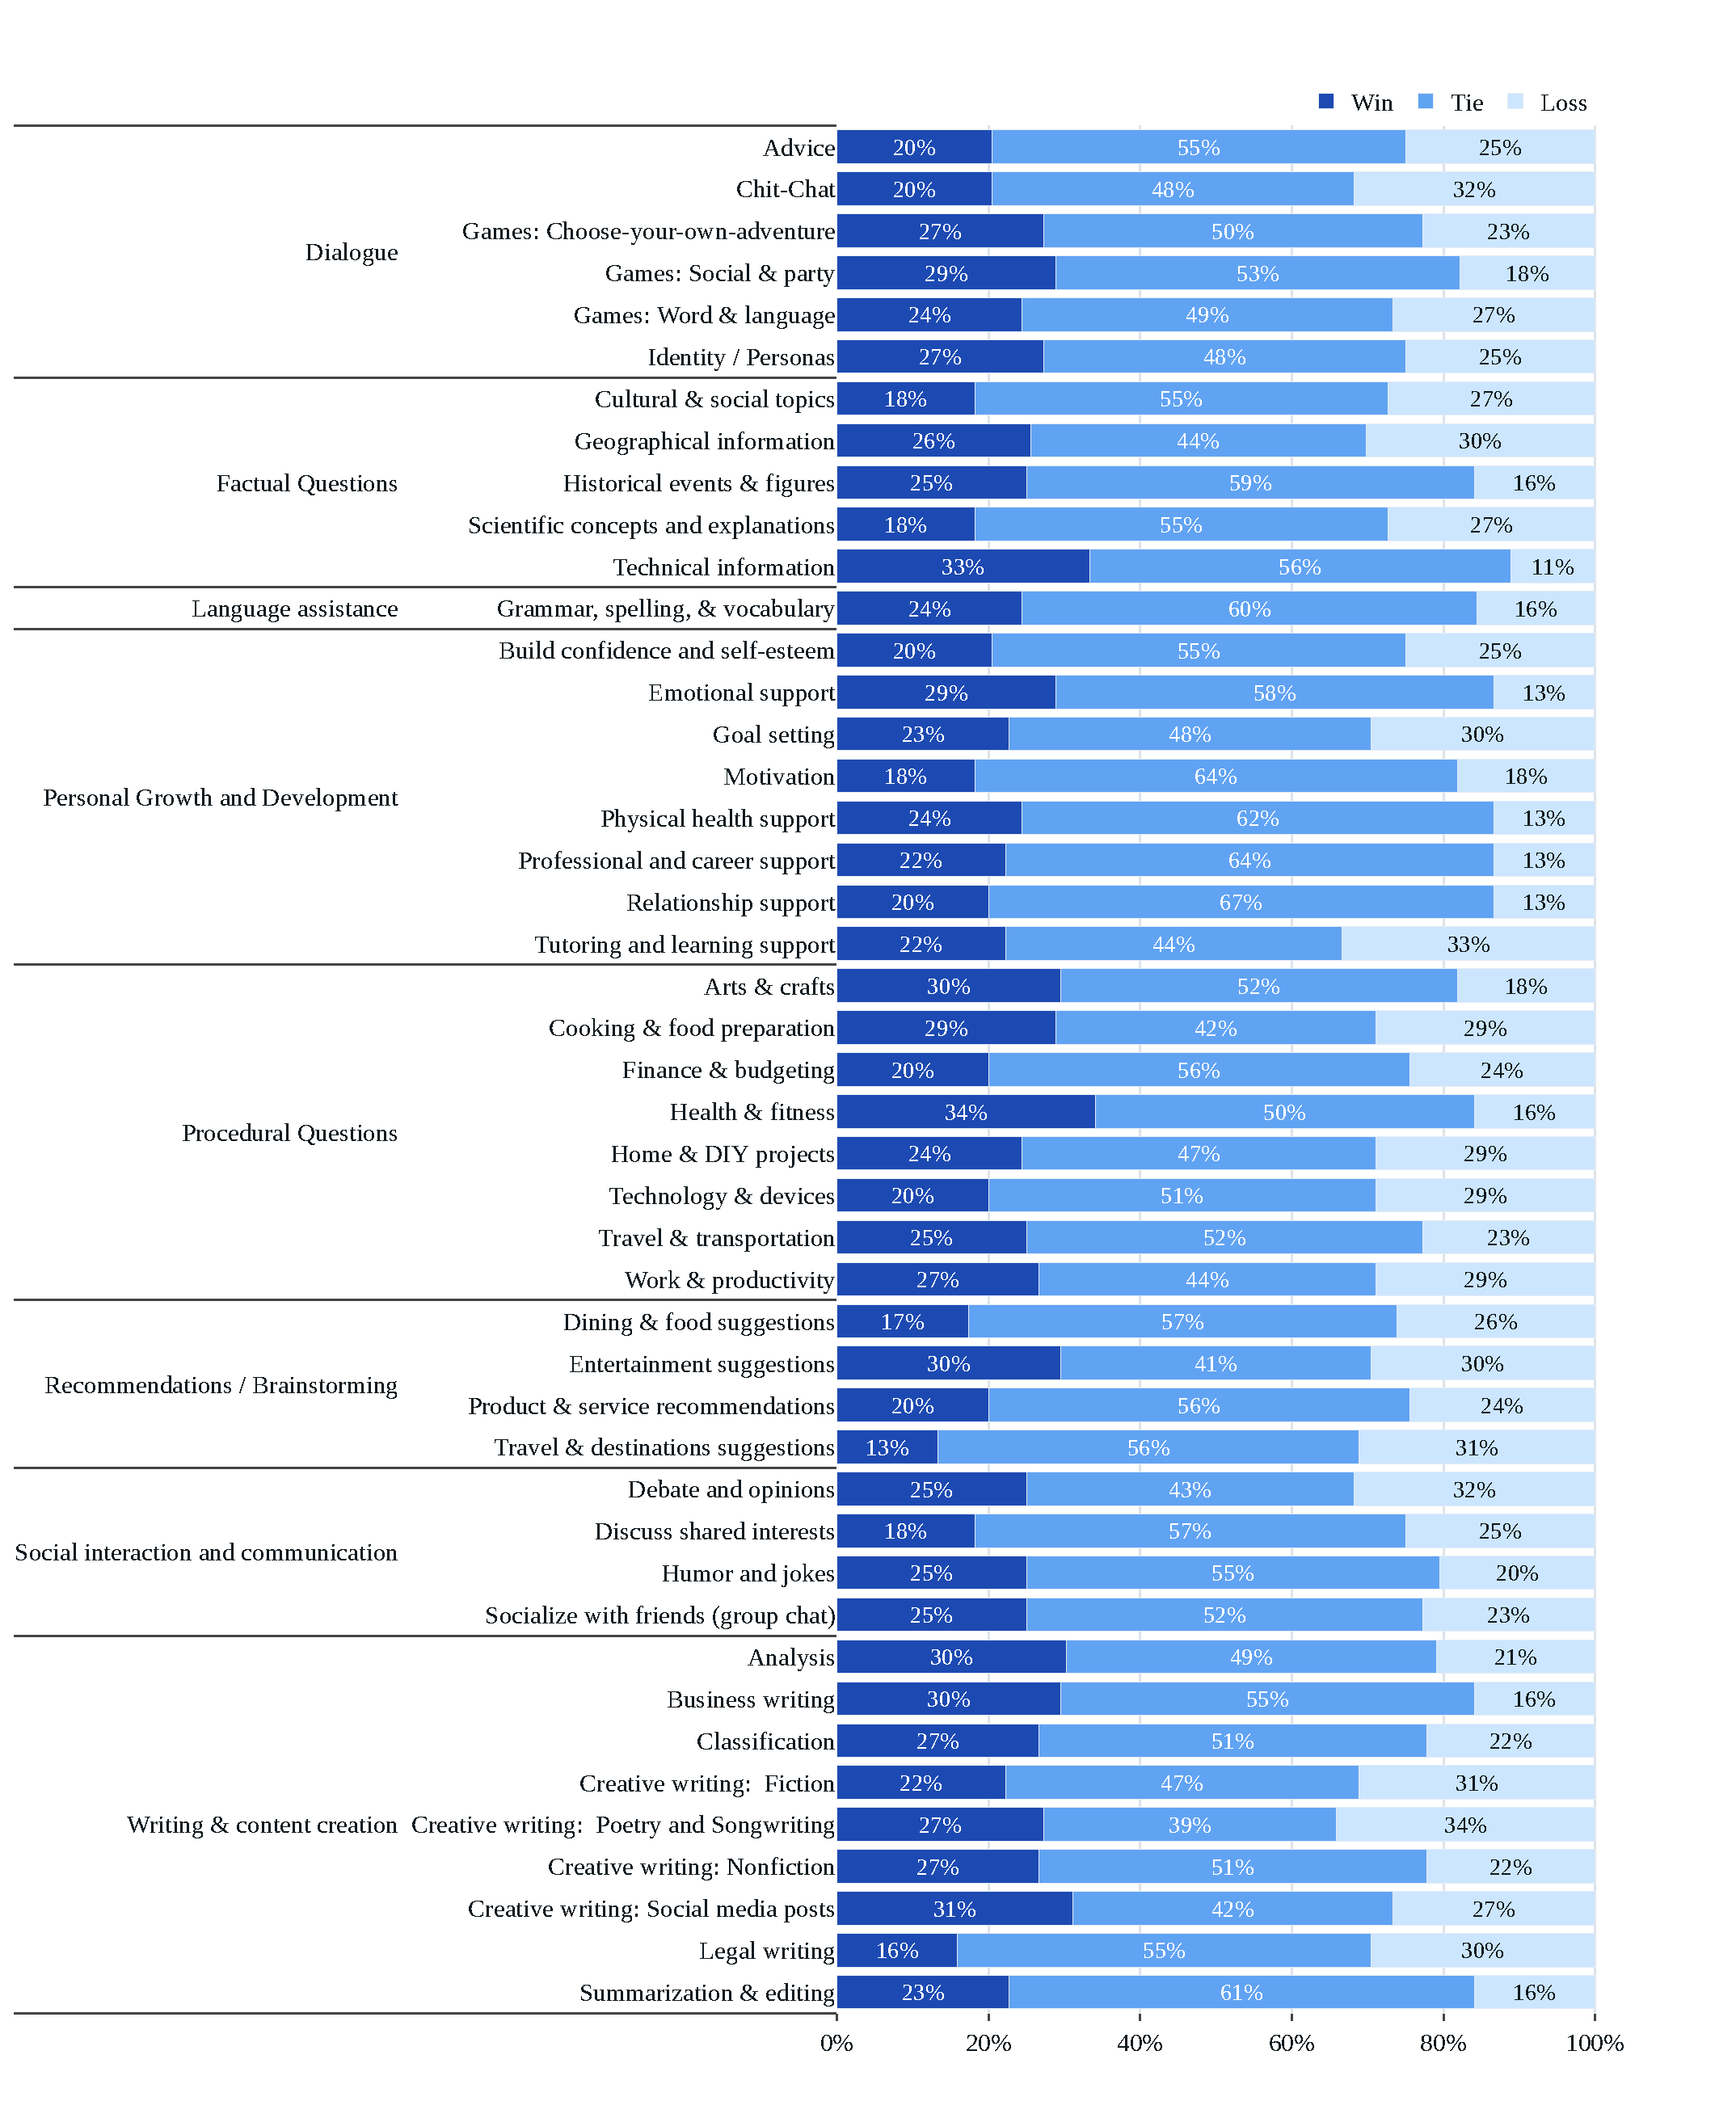
\includegraphics[width=0.75\linewidth]{assets/heval-gpt4preview-english-l2.pdf}
    \caption{Human evaluation results comparing the English capability of Llama 3 405B vs. GPT-4 across subcategories.}
    \label{fig:heval-gpt4o-english-l2.png}
\end{figure}



\begin{figure}
  \centering
  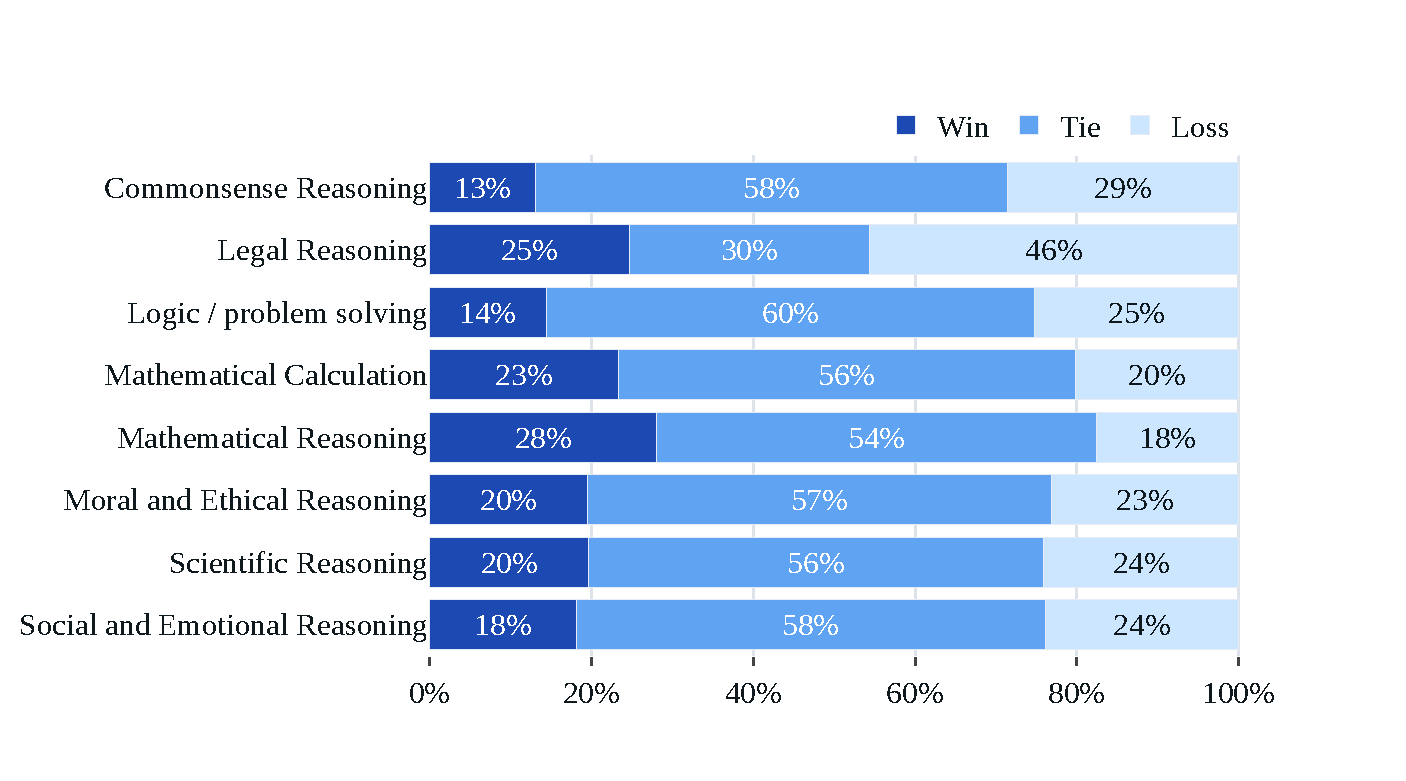
\includegraphics[width=0.75\linewidth]{assets/heval-gpt4preview-reasoning-l1.pdf}
  \caption{Human evaluation results comparing the reasoning capability of Llama 3 405B vs. GPT-4 across categories.}
  \label{fig:heval-gpt4o-reasoning-l1.png}
\end{figure}


\begin{figure}
  \centering
  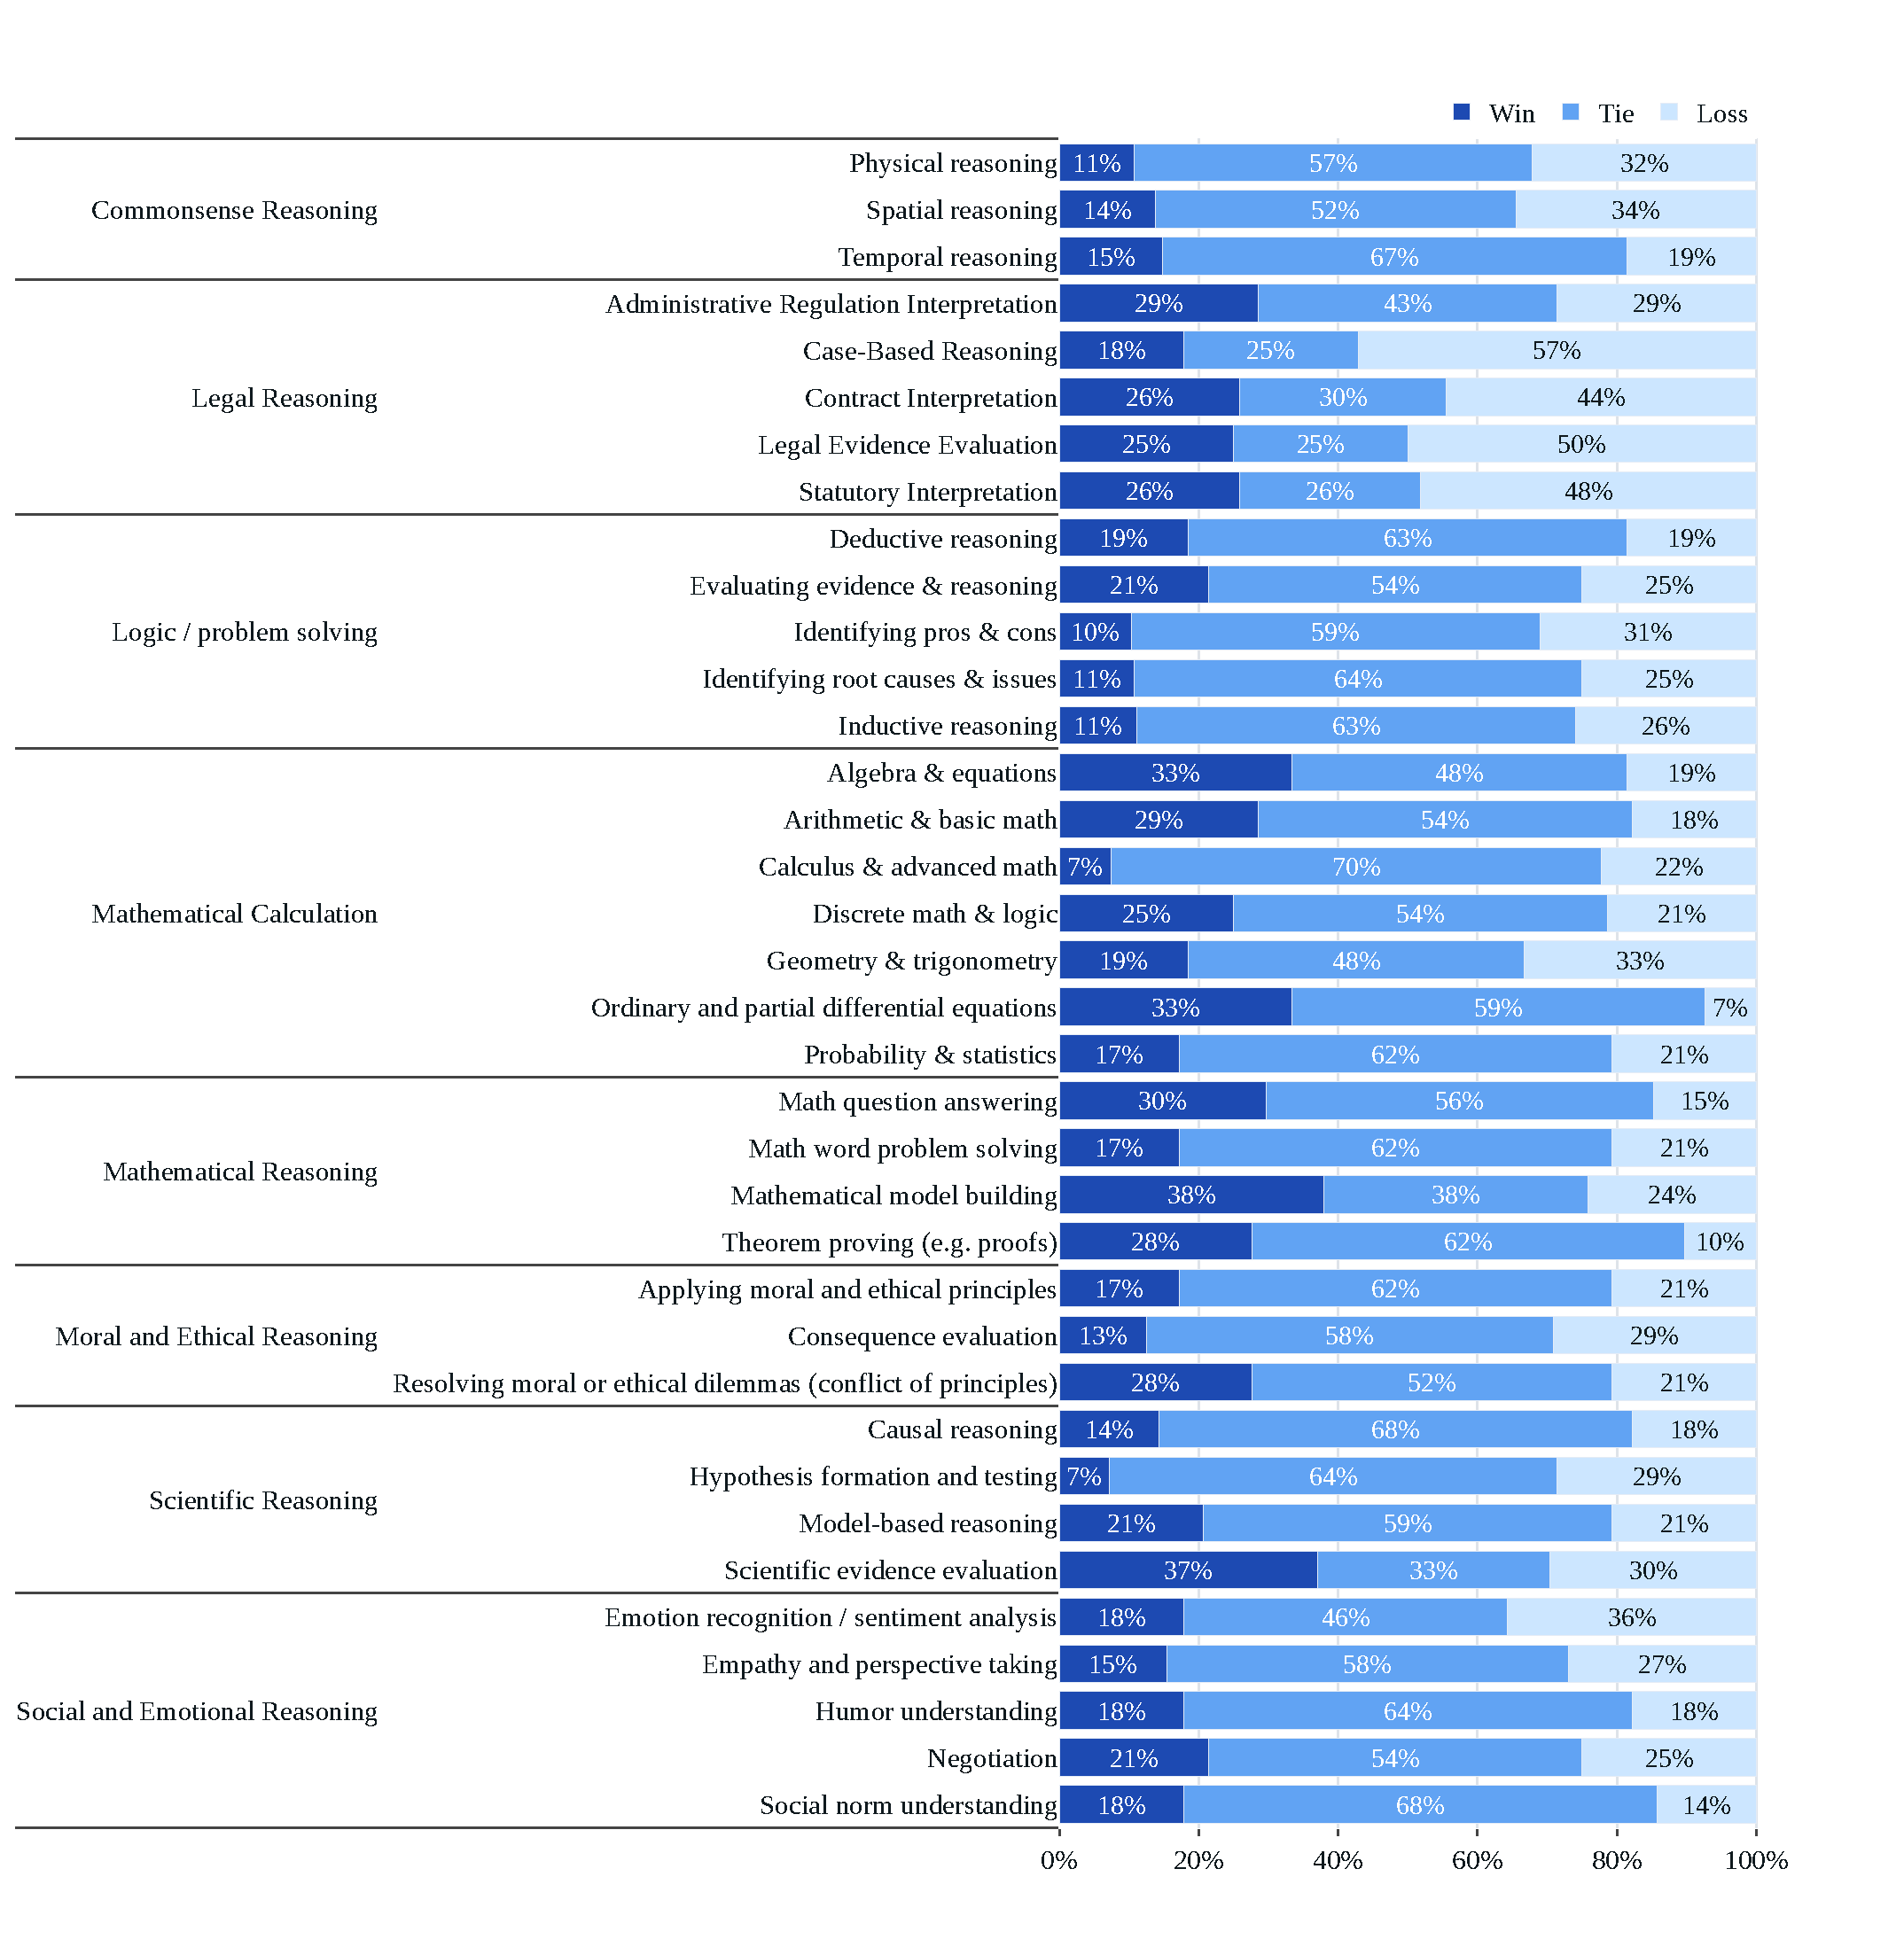
\includegraphics[width=0.75\linewidth]{assets/heval-gpt4preview-reasoning-l2.pdf}
  \caption{Human evaluation results comparing the reasoning capability of Llama 3 405B vs. GPT-4 across subcategories.}
  \label{fig:heval-gpt4o-reasoning-l2.png}
\end{figure}


\begin{figure}
  \centering
  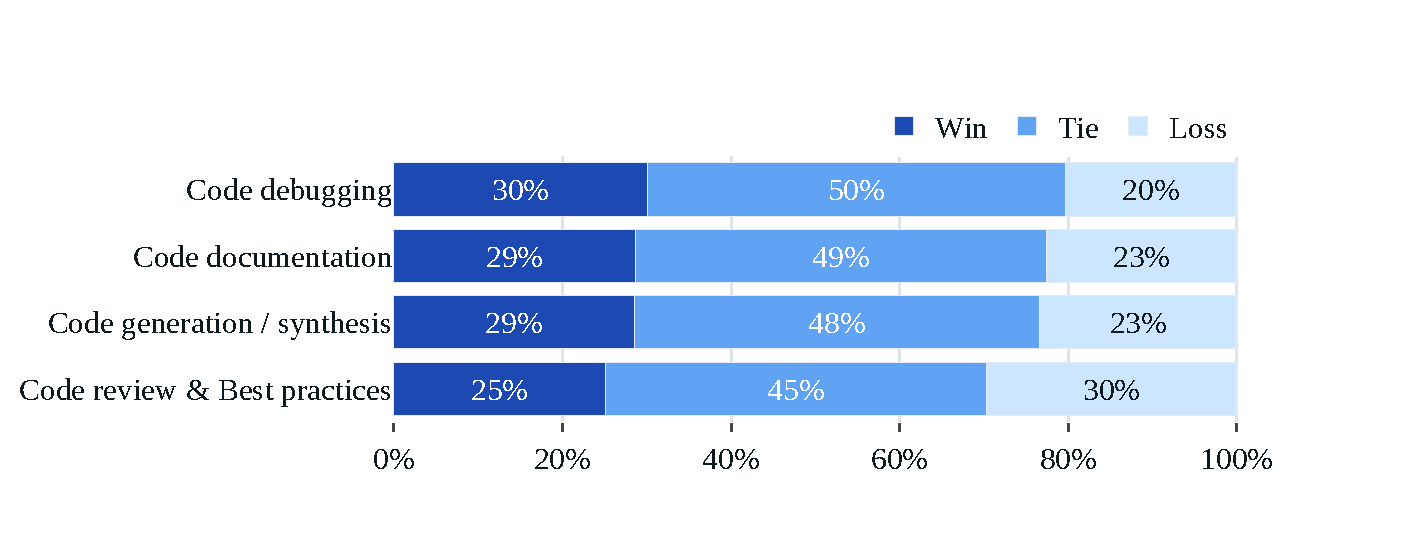
\includegraphics[width=0.75\linewidth]{assets/heval-gpt4preview-coding-l1.pdf}
  \caption{Human evaluation results comparing the coding capability of Llama 3 405B vs. GPT-4 across categories.}
  \label{fig:heval-gpt4o-coding-l1.png}
\end{figure}


\begin{figure}
  \centering
  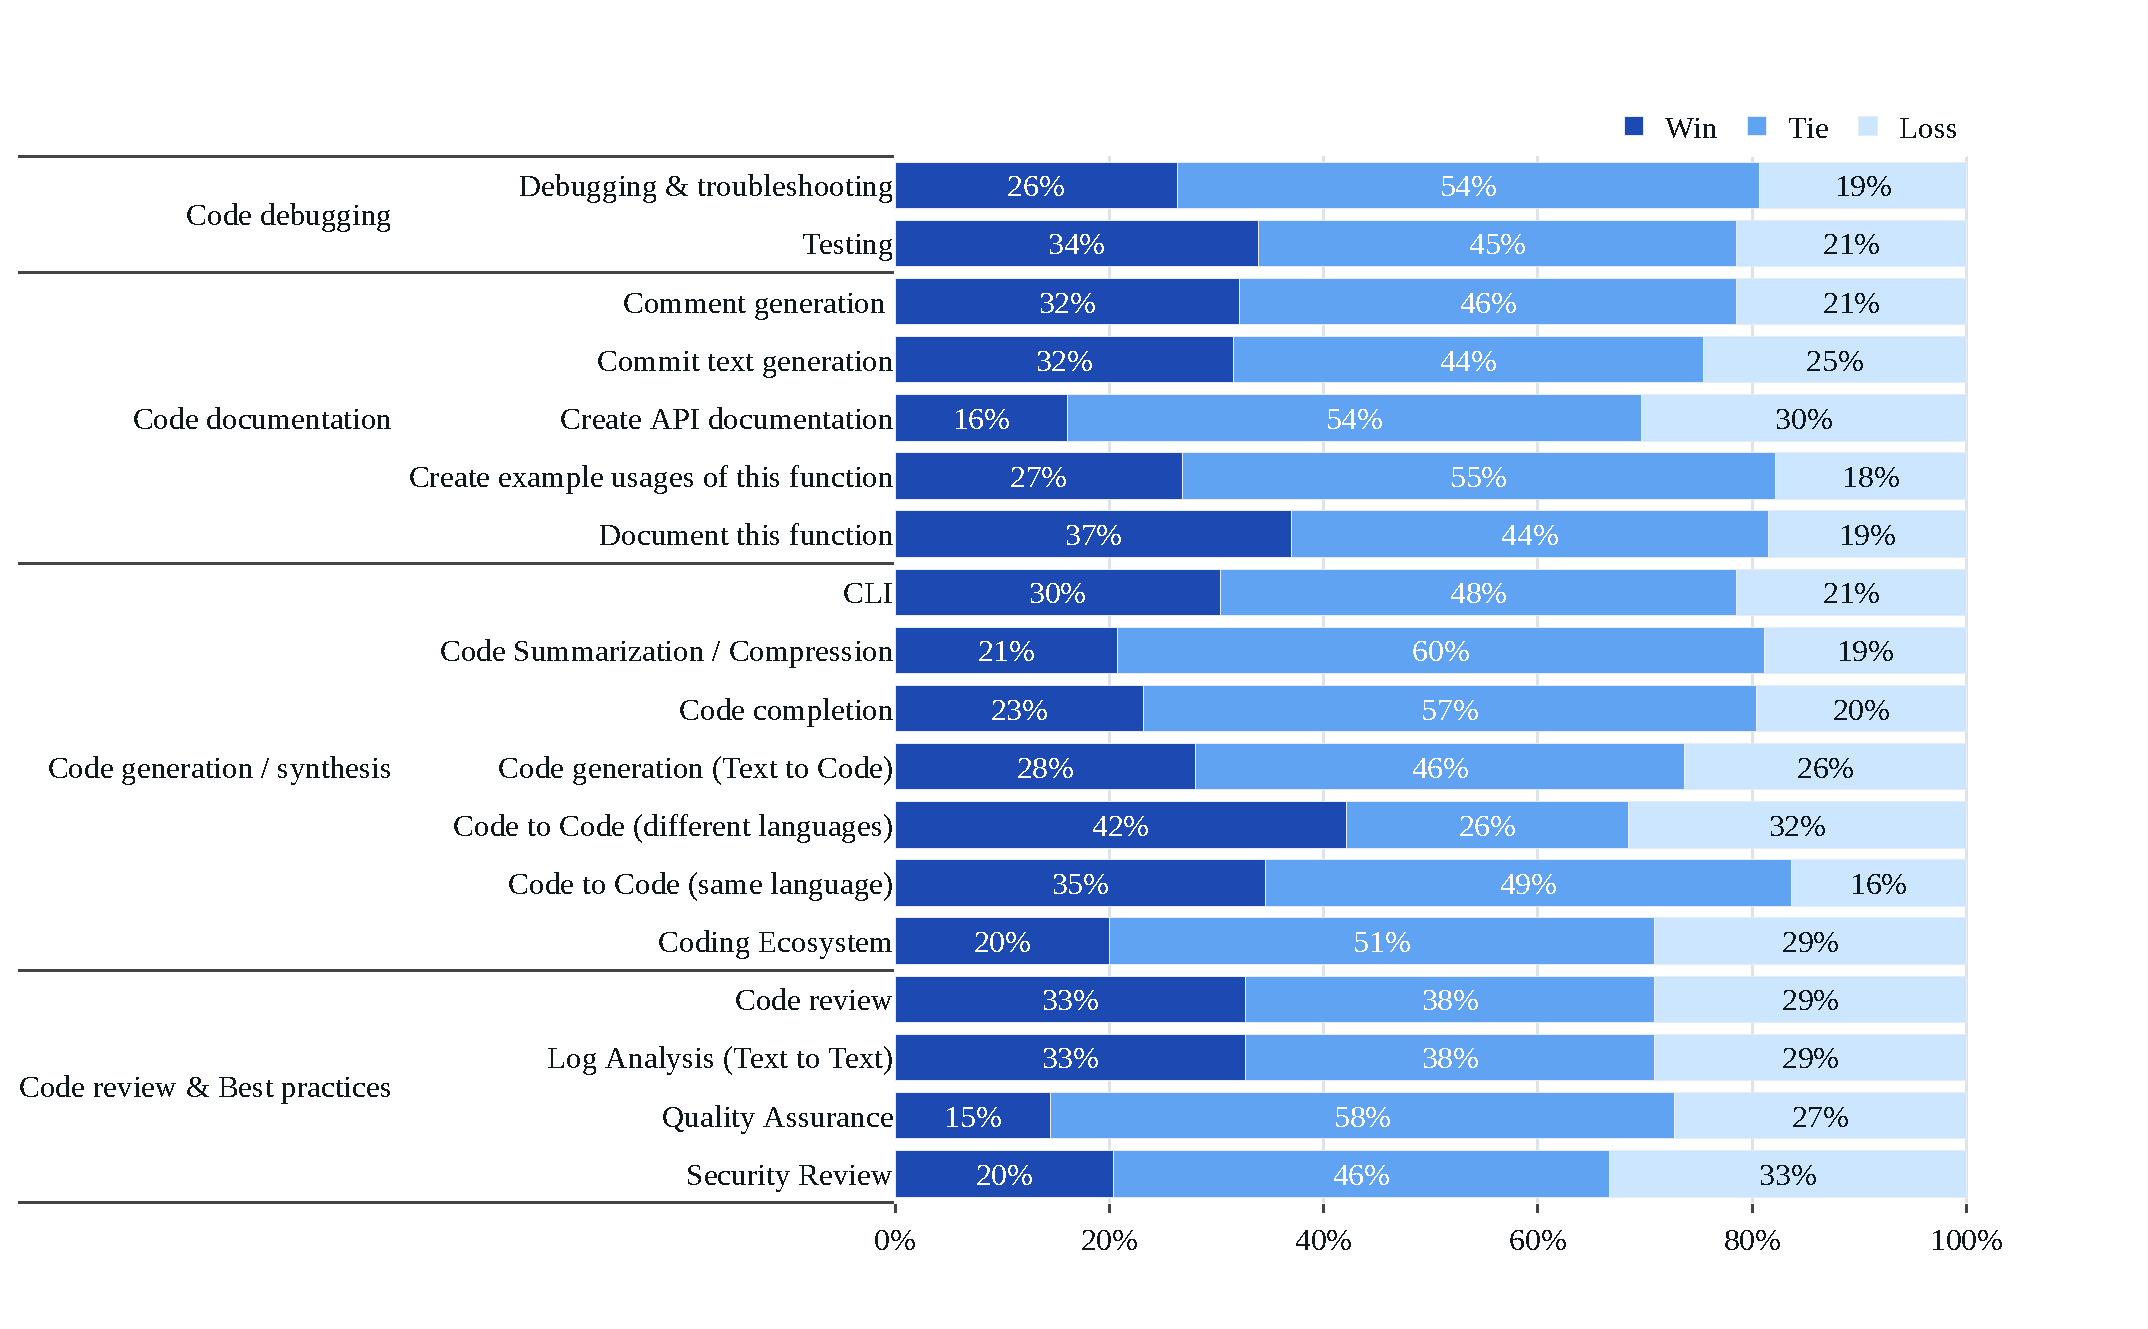
\includegraphics[width=0.75\linewidth]{assets/heval-gpt4preview-coding-l2.pdf}
  \caption{Human evaluation results comparing the coding capability of Llama 3 405B vs. GPT-4 across subcategories.}
  \label{fig:heval-gpt4o-coding-l2.png}
\end{figure}




\begin{figure}
    \centering
    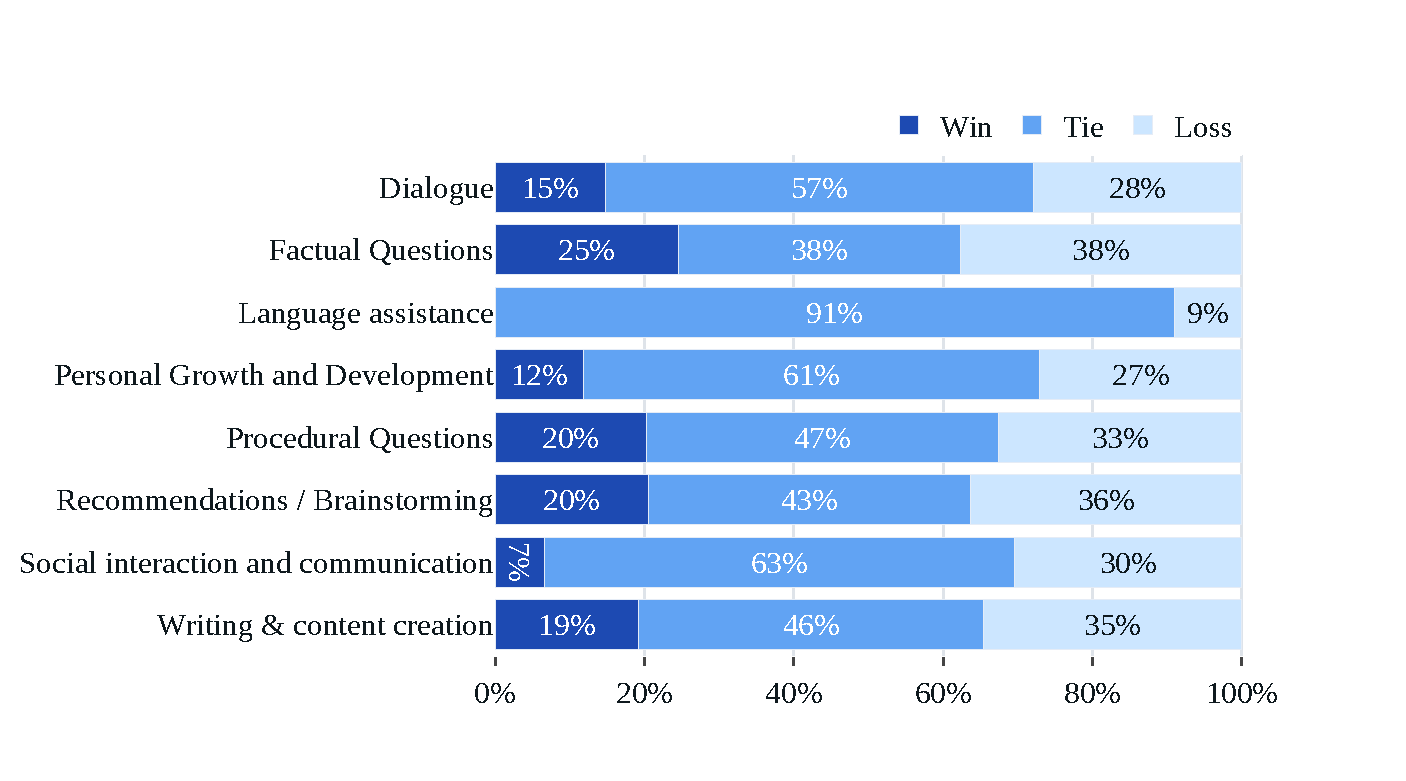
\includegraphics[width=0.75\linewidth]{assets/heval-gpt4preview-hindi-l1.pdf}
    \caption{Human evaluation results comparing the Hindi capability of Llama 3 405B vs. GPT-4 across categories.}
    \label{fig:heval-gpt4o-hindi-l1.png}
\end{figure}


\begin{figure}
    \centering
    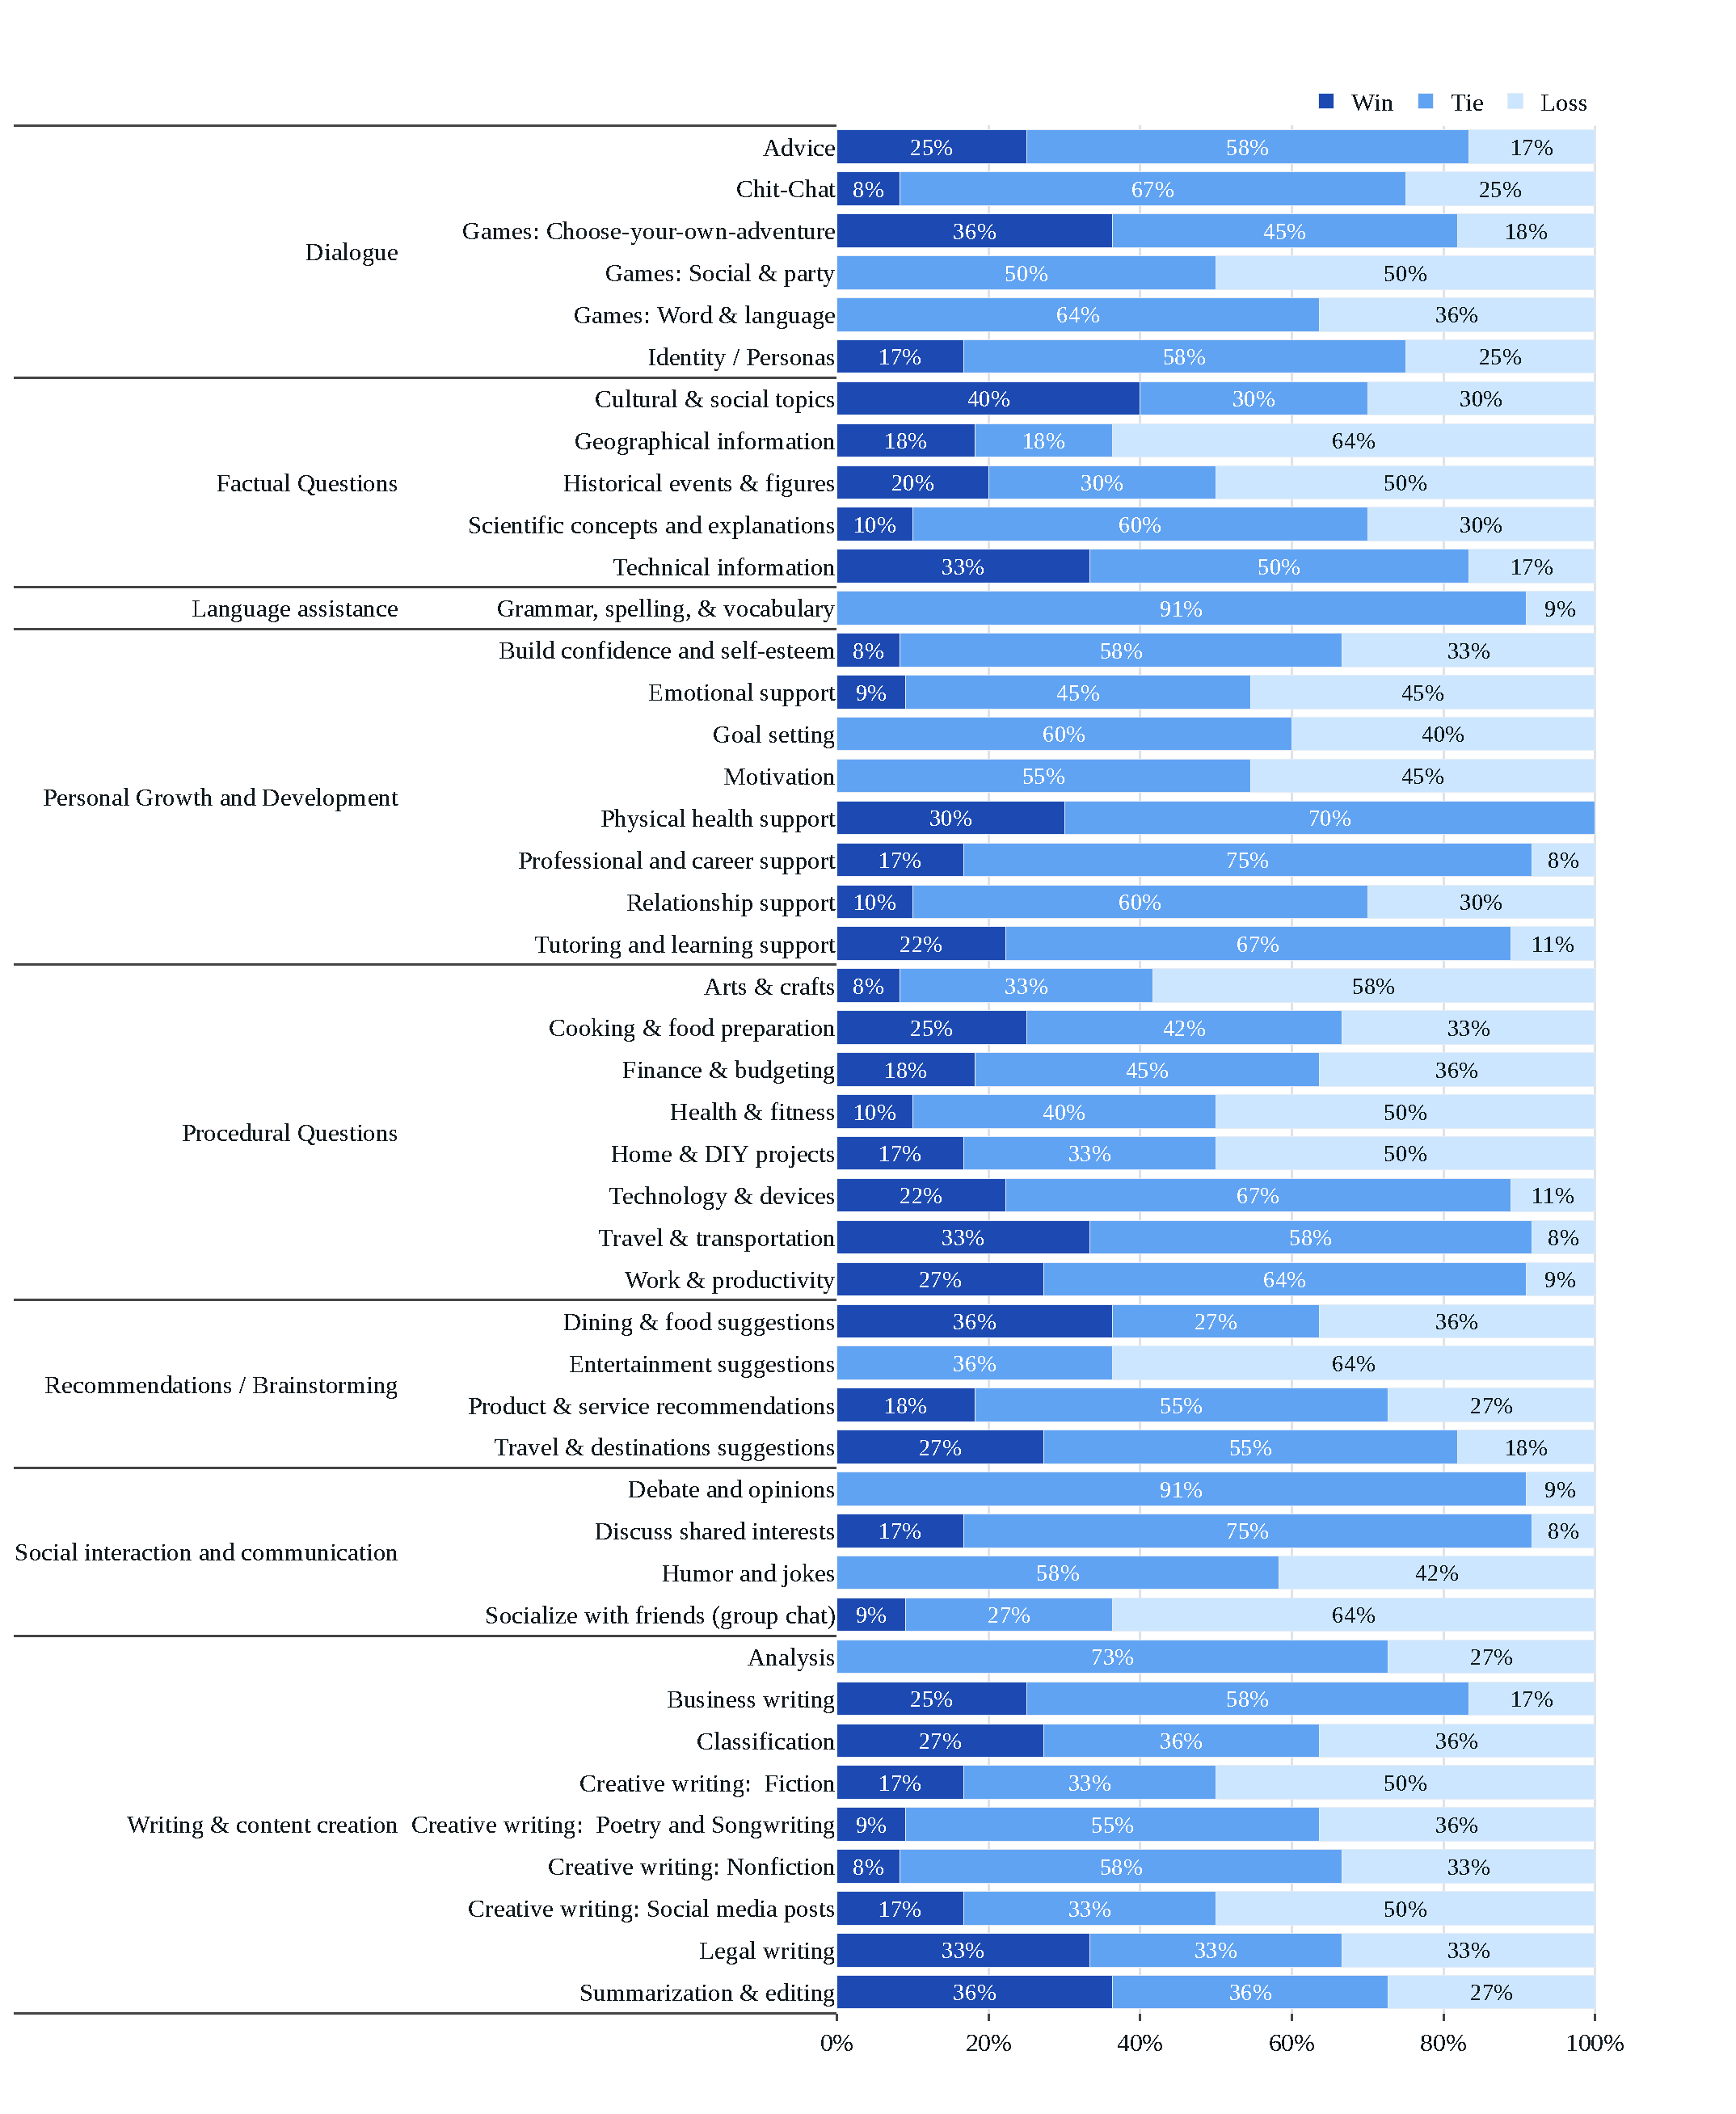
\includegraphics[width=0.75\linewidth]{assets/heval-gpt4preview-hindi-l2.pdf}
    \caption{Human evaluation results comparing the Hindi capability of Llama 3 405B vs. GPT-4 across subcategories.}
    \label{fig:heval-gpt4o-hindi-l2.png}
\end{figure}


\begin{figure}
    \centering
    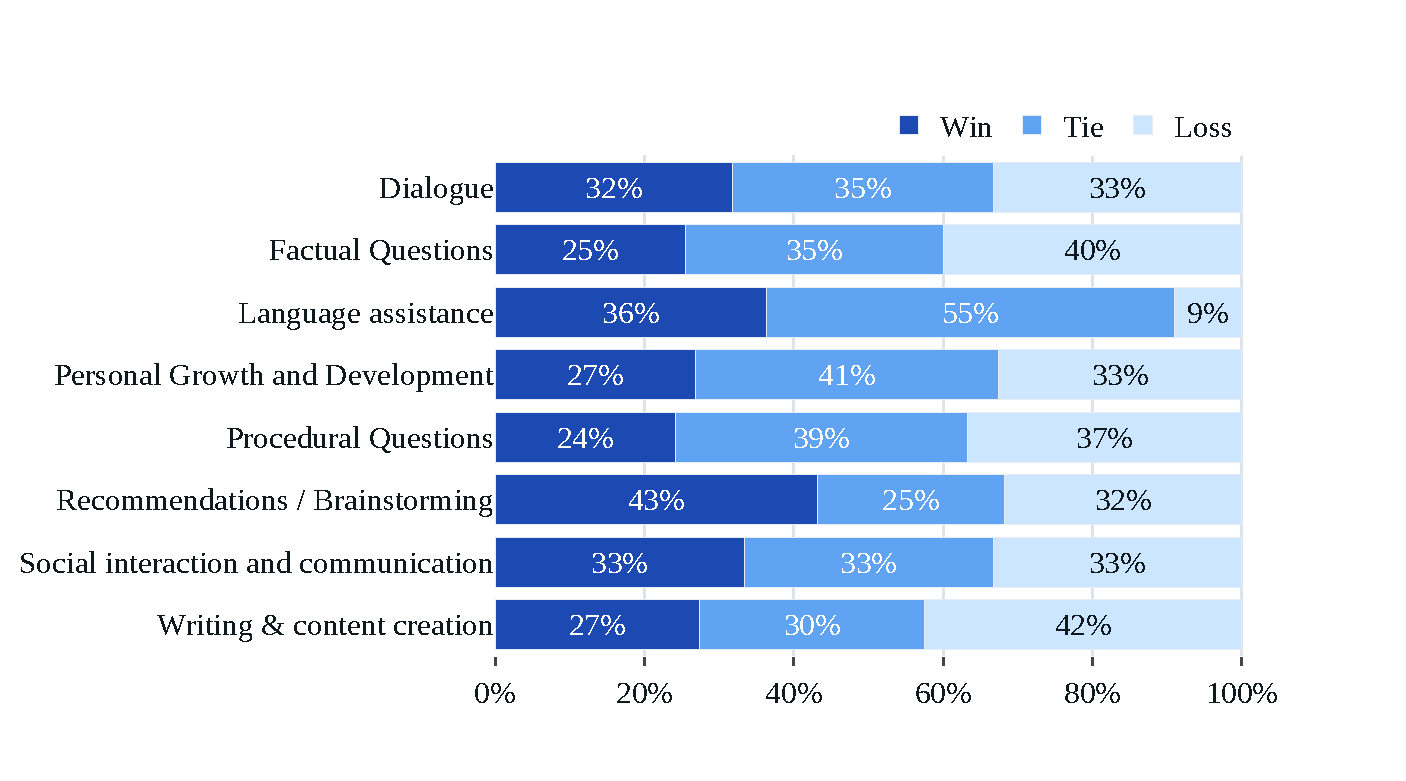
\includegraphics[width=0.75\linewidth]{assets/heval-gpt4preview-spanish-l1.pdf}
    \caption{Human evaluation results comparing the Spanish capability of Llama 3 405B vs. GPT-4 across categories.}
    \label{fig:heval-gpt4o-spanish-l1.png}
\end{figure}


\begin{figure}
    \centering
    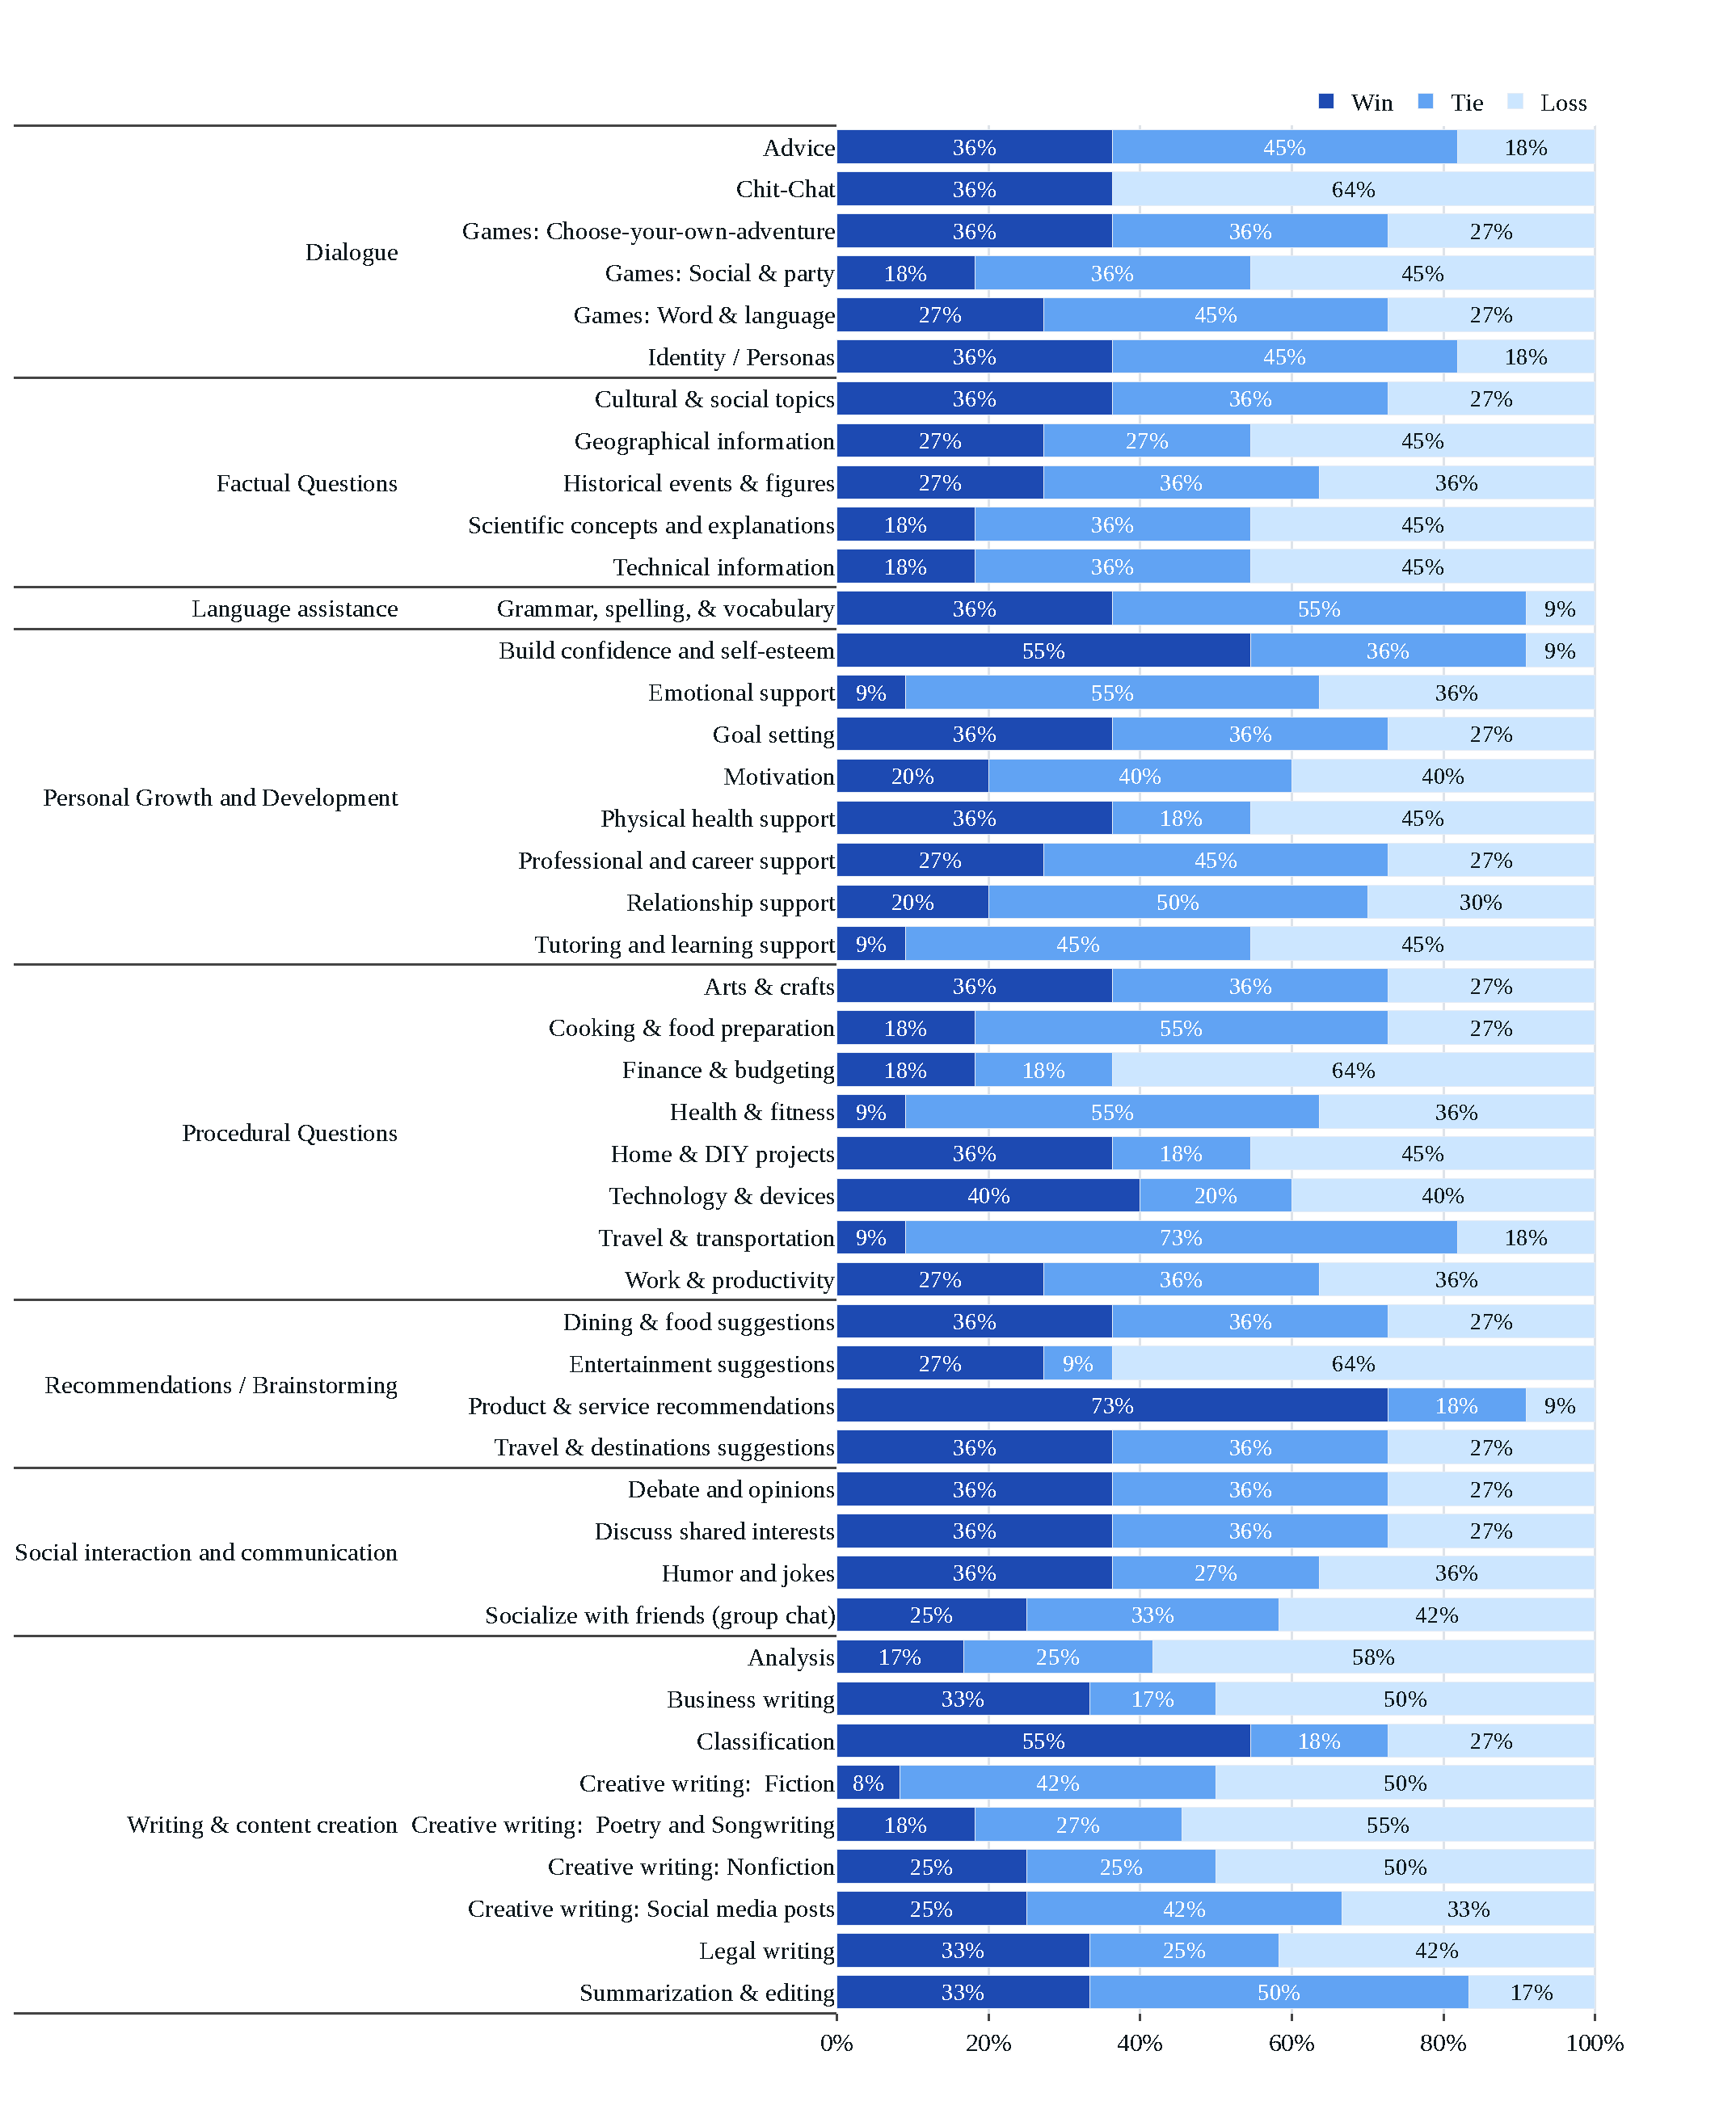
\includegraphics[width=0.75\linewidth]{assets/heval-gpt4preview-spanish-l2.pdf}
    \caption{Human evaluation results comparing the Spanish capability of Llama 3 405B vs. GPT-4 across subcategories.}
    \label{fig:heval-gpt4o-spanish-l2.png}
\end{figure}

\begin{figure}
    \centering
    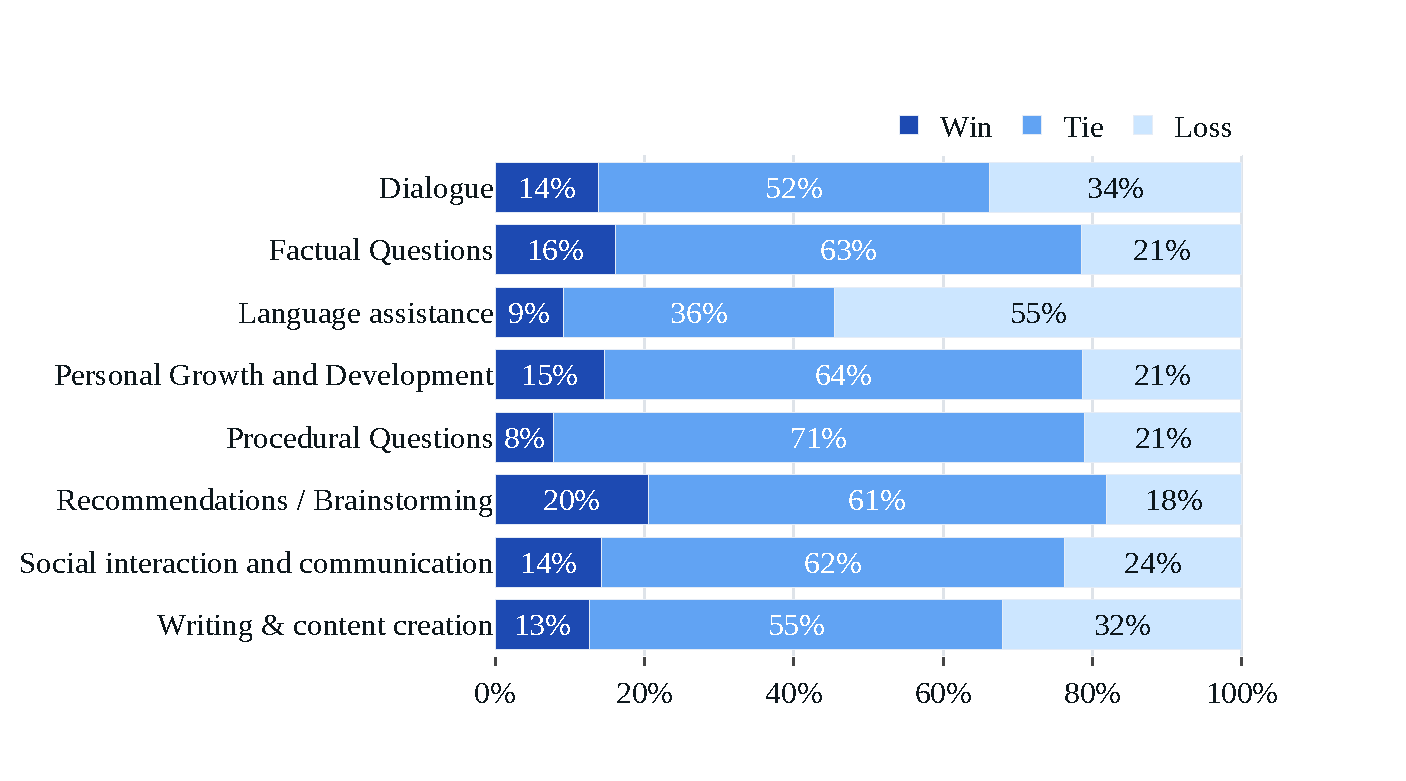
\includegraphics[width=0.75\linewidth]{assets/heval-gpt4preview-portuguese-l1.pdf}
    \caption{Human evaluation results comparing the Portuguese capability of Llama 3 405B vs. GPT-4 across categories.}
    \label{fig:heval-gpt4o-portuguese-l1.png}
\end{figure}


\begin{figure}
    \centering
    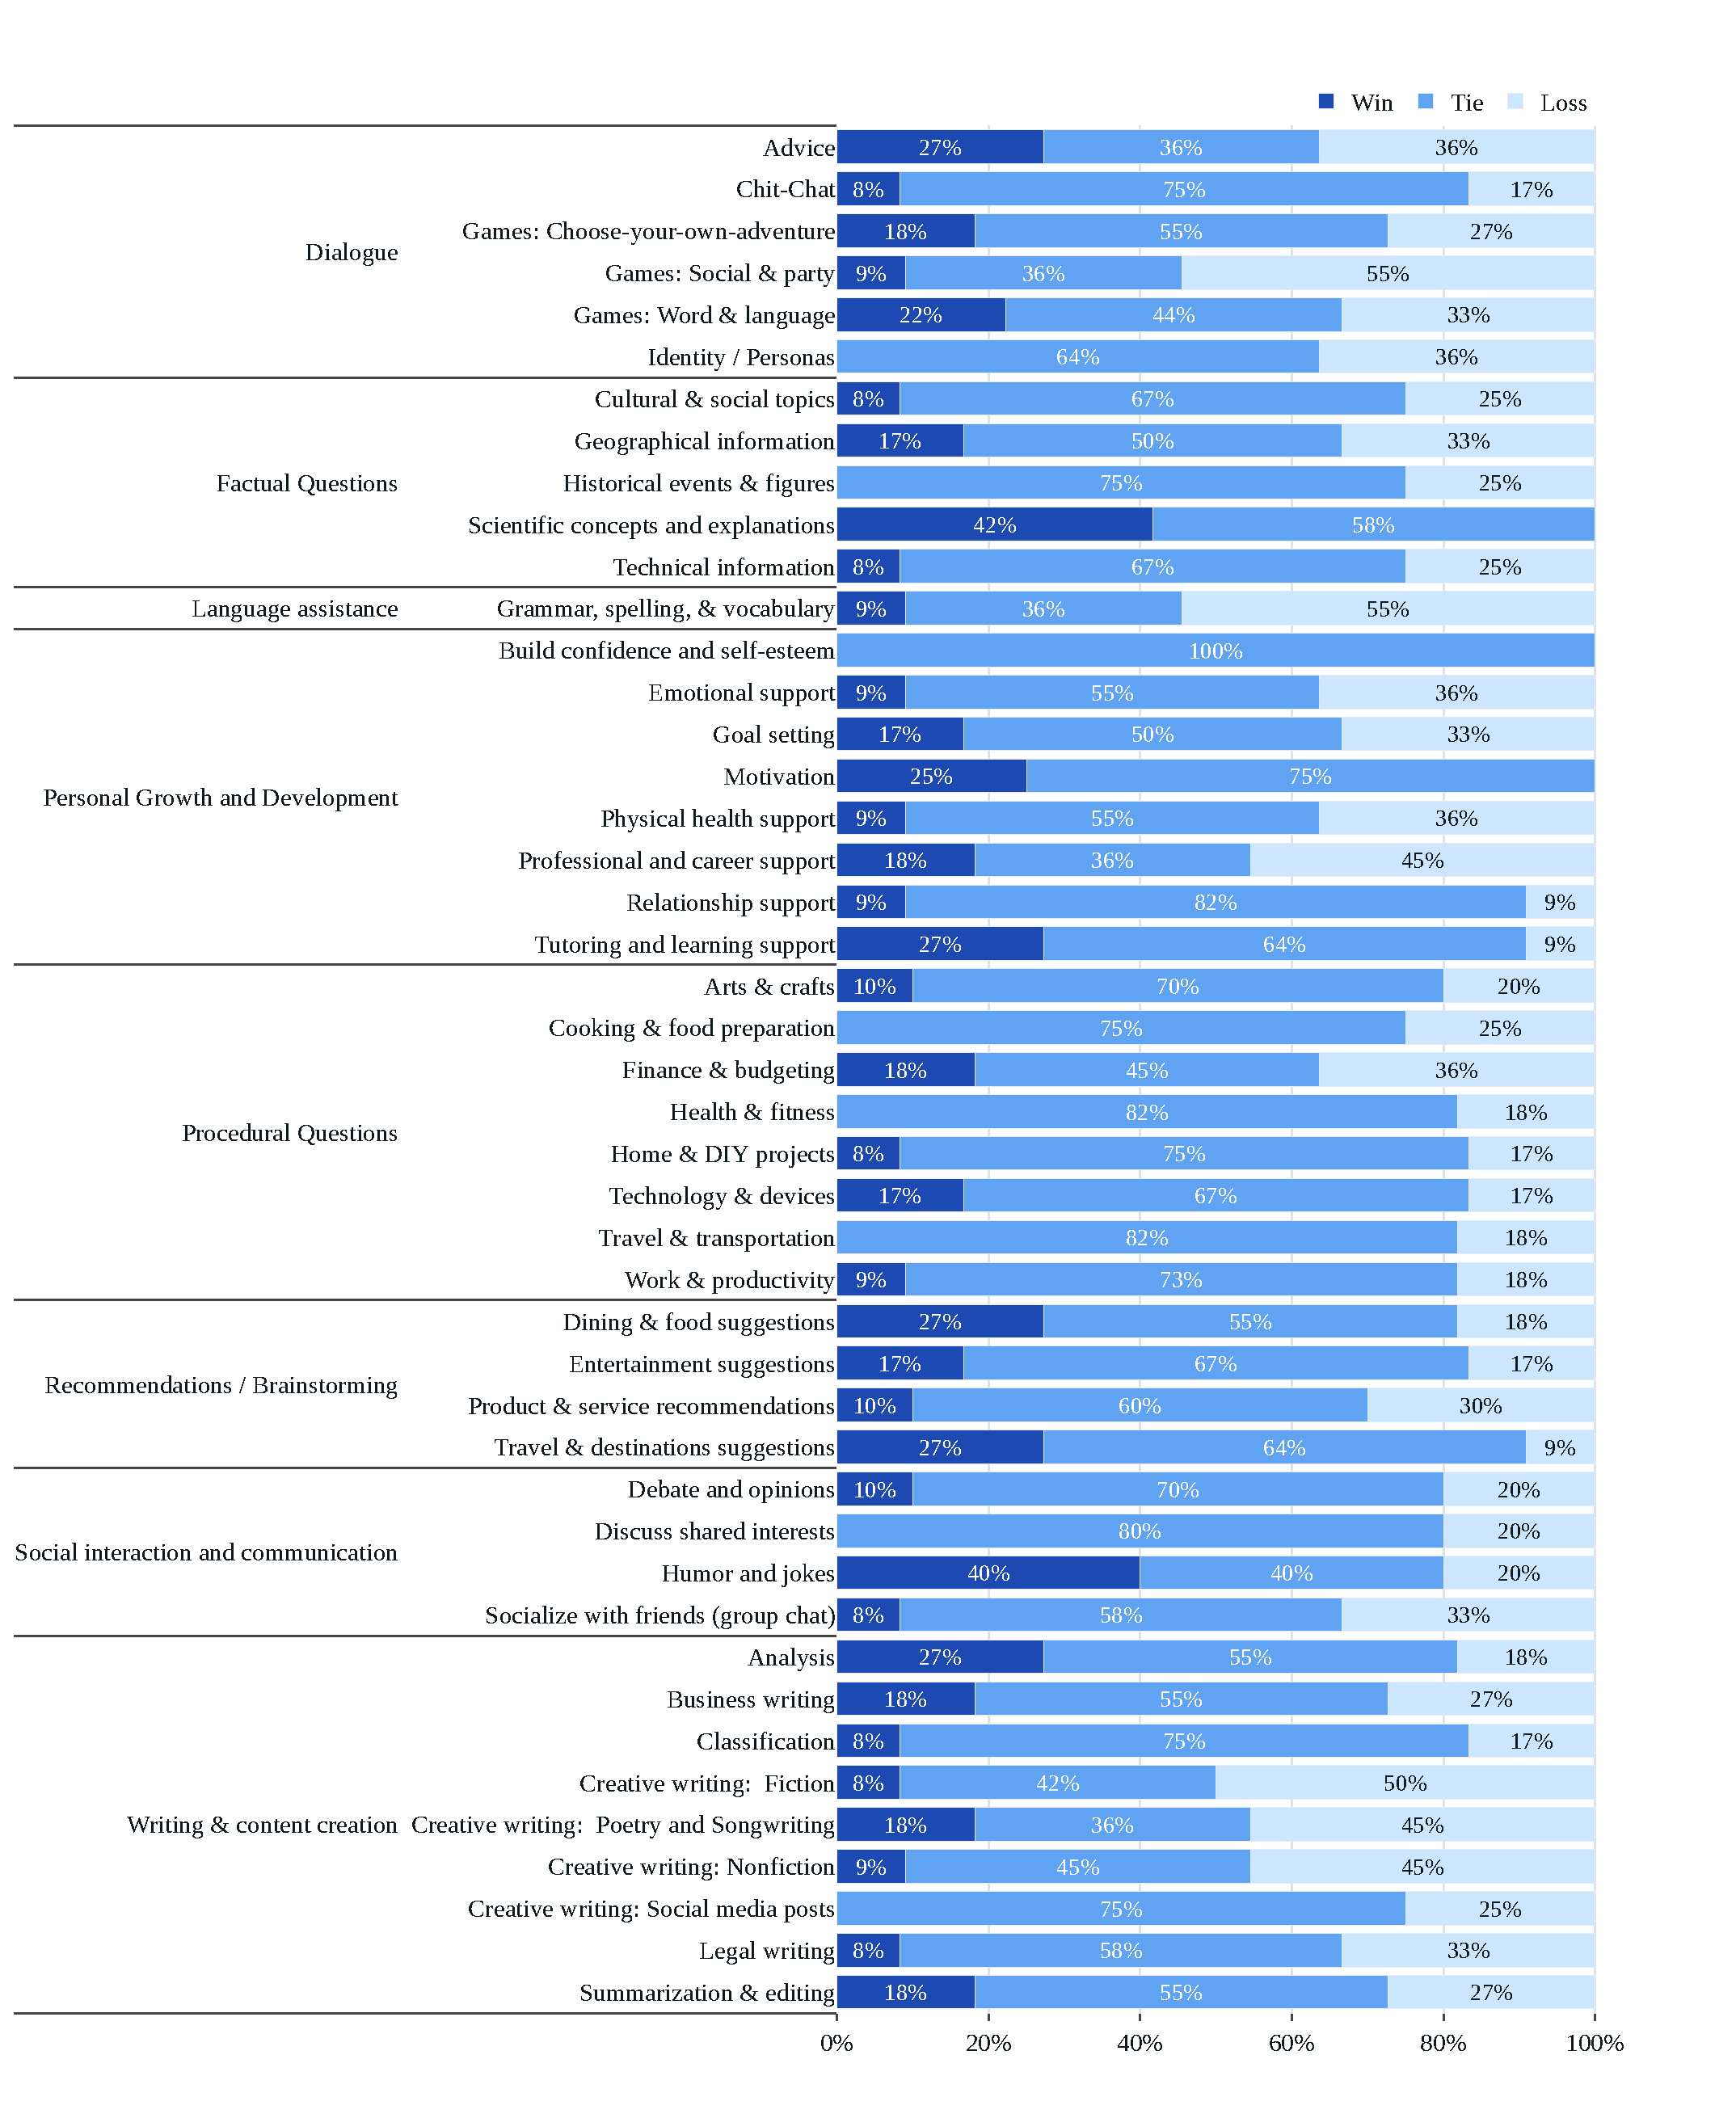
\includegraphics[width=0.75\linewidth]{assets/heval-gpt4preview-portuguese-l2.pdf}
    \caption{Human evaluation results comparing the Portuguese capability of Llama 3 405B vs. GPT-4 across subcategories.}
    \label{fig:heval-gpt4o-portuguese-l2.png}
\end{figure}









\begin{figure}
    \centering
    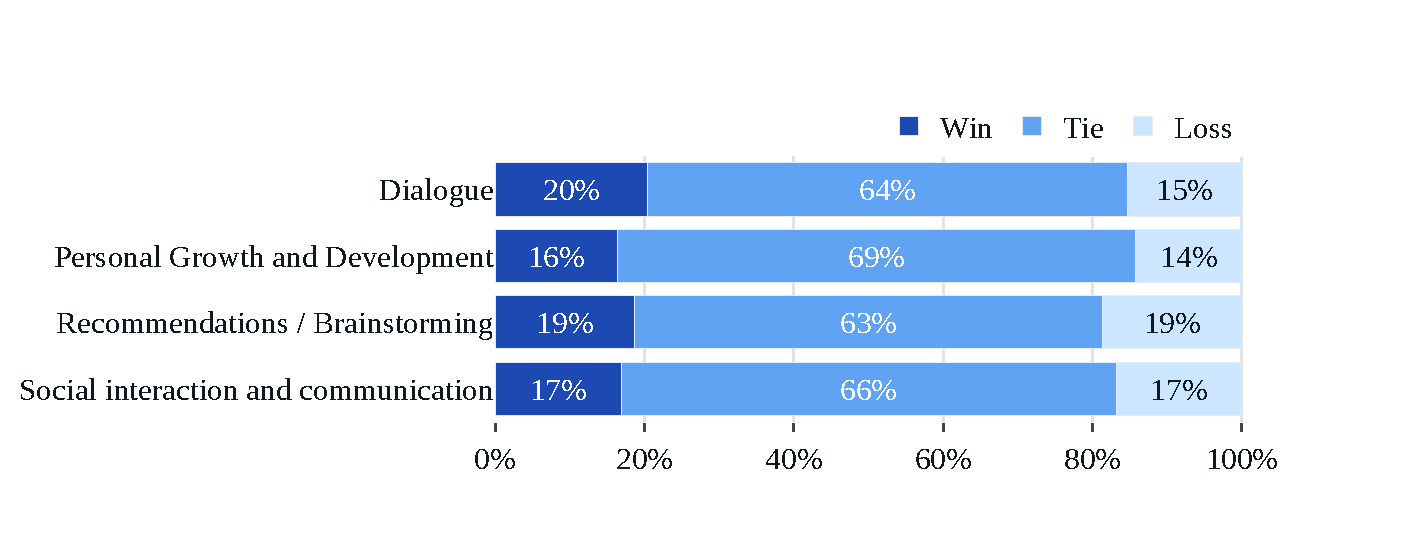
\includegraphics[width=0.75\linewidth]{assets/heval-gpt4preview-multiturn-english-l1.pdf}
    \caption{Human evaluation results comparing the multiturn English capability of Llama 3 405B vs. GPT-4 across categories.}
    \label{fig:heval-gpt4o-multiturn-english-l1.png}
\end{figure}


\begin{figure}
    \centering
    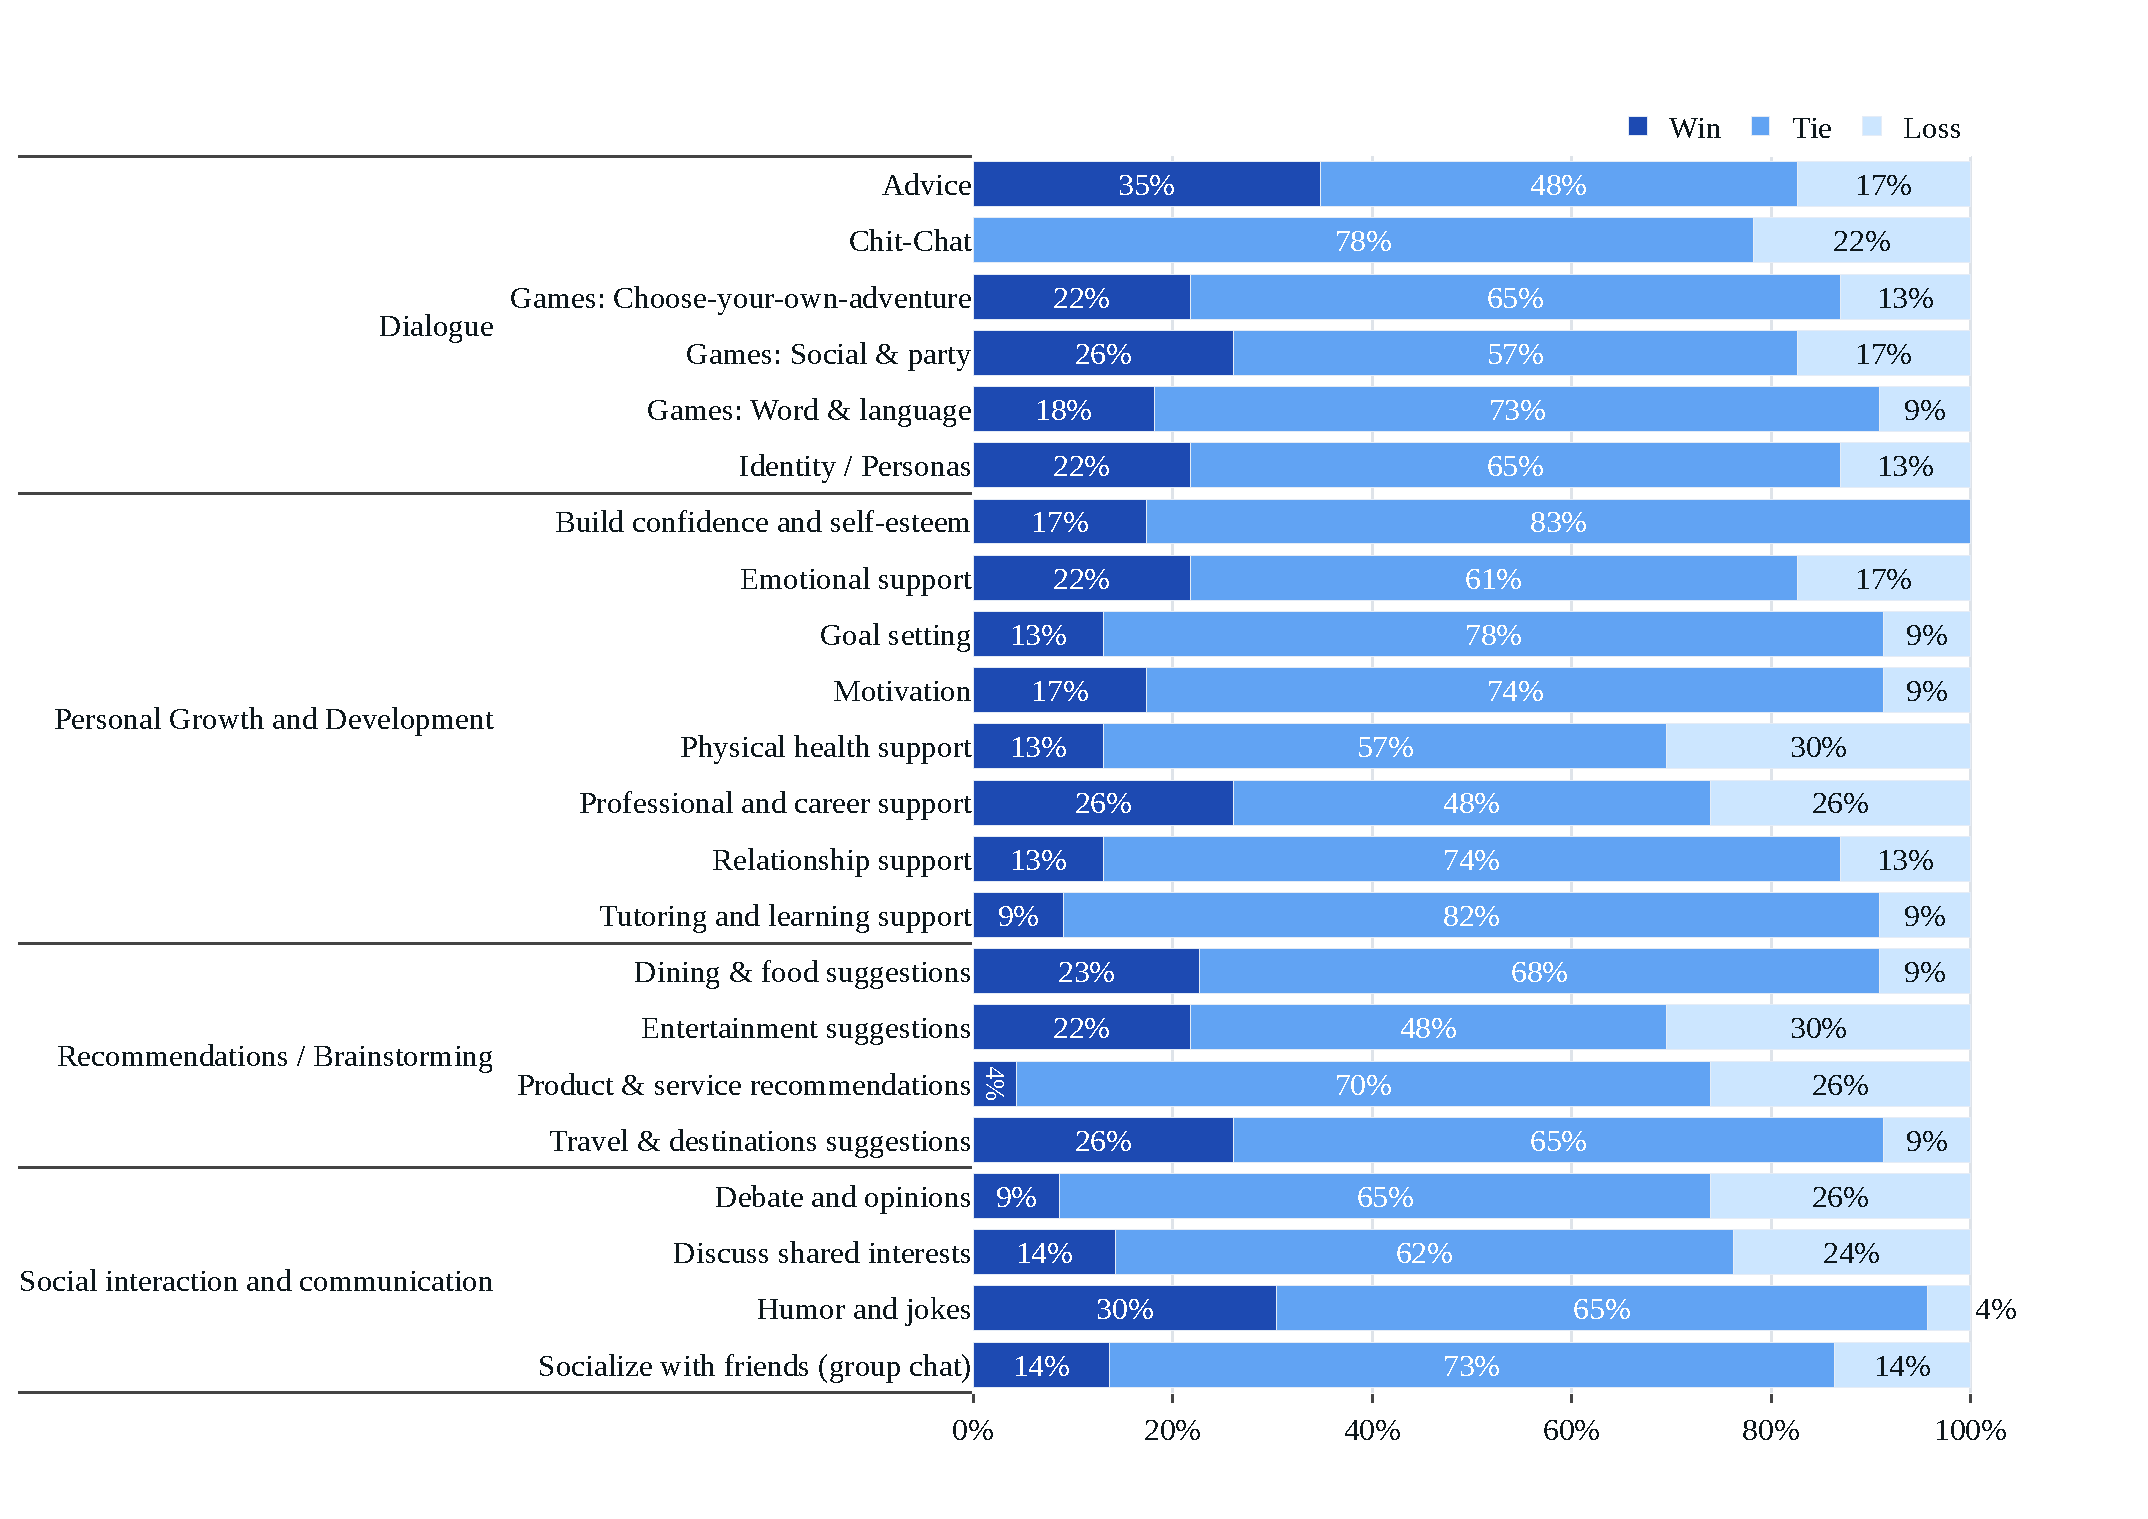
\includegraphics[width=0.75\linewidth]{assets/heval-gpt4preview-multiturn-english-l2.pdf}
    \caption{Human evaluation results comparing the multiturn English capability of Llama 3 405B vs. GPT-4 across subcategories.}
    \label{fig:heval-gpt4o-multiturn-english-l2.png}
\end{figure}

\begin{figure}
    \centering
    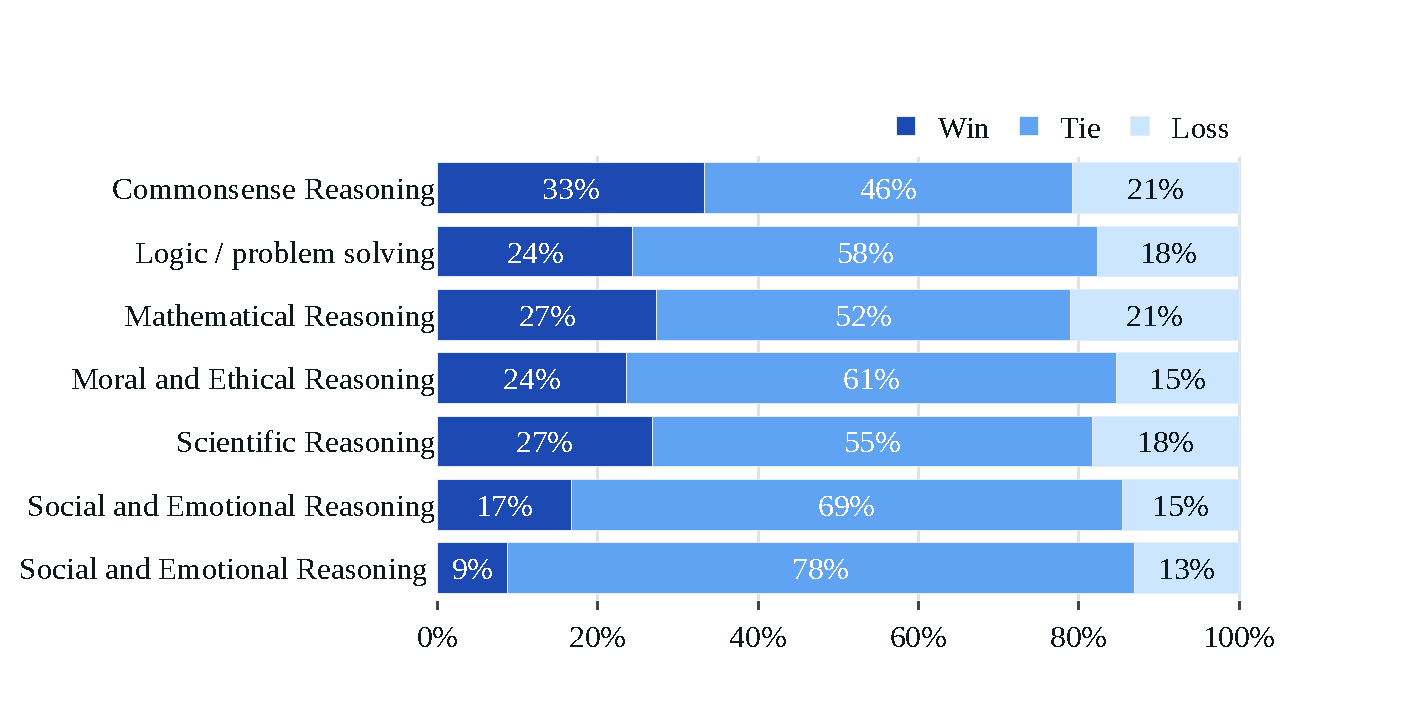
\includegraphics[width=0.75\linewidth]{assets/heval-gpt4preview-multiturn-reasoning-l1.pdf}
    \caption{Human evaluation results comparing the multiturn reasoning capability of Llama 3 405B vs. GPT-4 across categories.}
    \label{fig:heval-gpt4o-multiturn-reasoning-l1.png}
\end{figure}


\begin{figure}
    \centering
    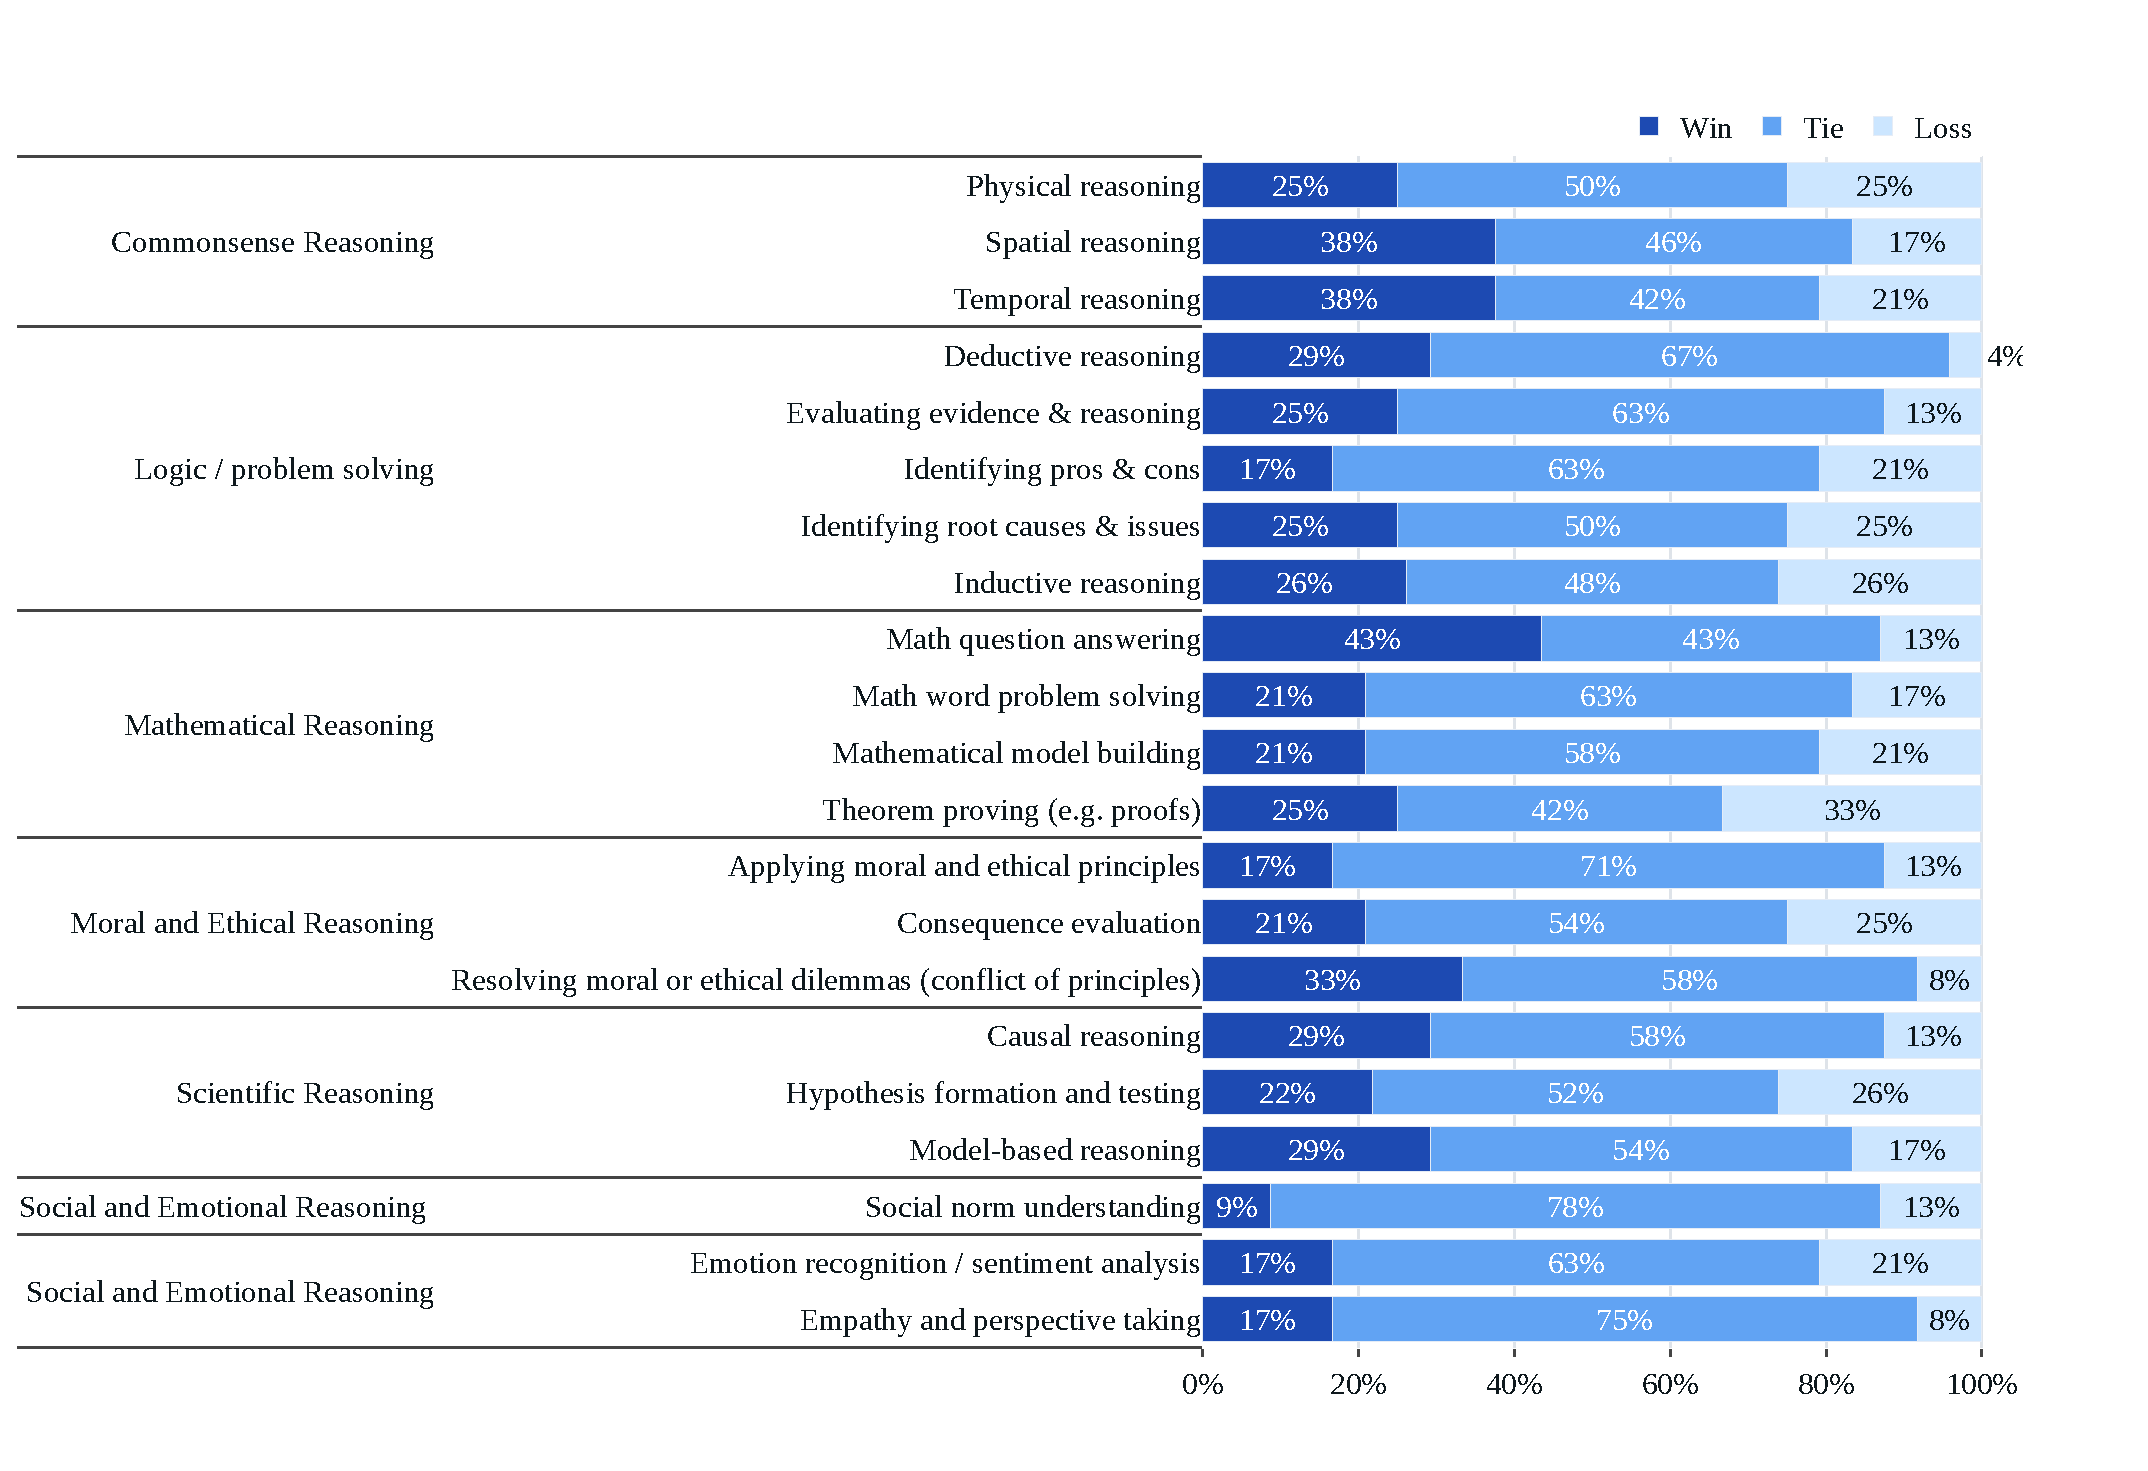
\includegraphics[width=0.75\linewidth]{assets/heval-gpt4preview-multiturn-reasoning-l2.pdf}
    \caption{Human evaluation results comparing the multiturn reasoning capability of Llama 3 405B vs. GPT-4 across subcategories.}
    \label{fig:heval-gpt4o-multiturn-reasoning-l2.png}
\end{figure}


\begin{figure}
    \centering
    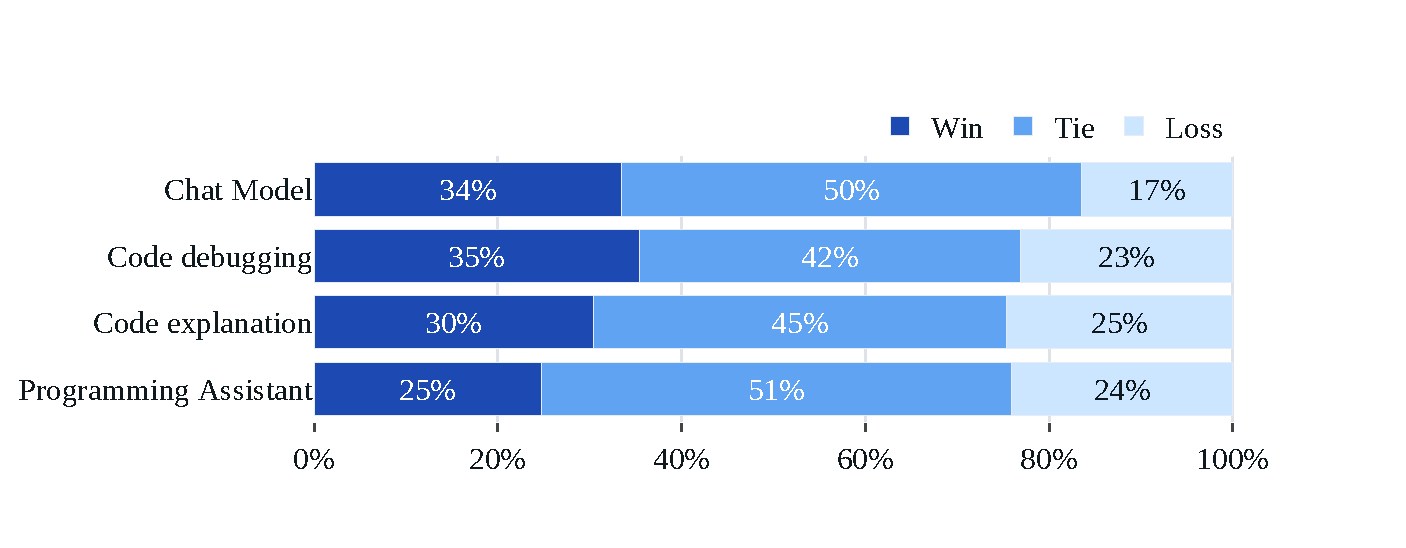
\includegraphics[width=0.75\linewidth]{assets/heval-gpt4preview-multiturn-coding-l1.pdf}
    \caption{Human evaluation results comparing the multiturn coding capability of Llama 3 405B vs. GPT-4 across categories.}
    \label{fig:heval-gpt4o-multiturn-coding-l1.png}
\end{figure}


\begin{figure}
    \centering
    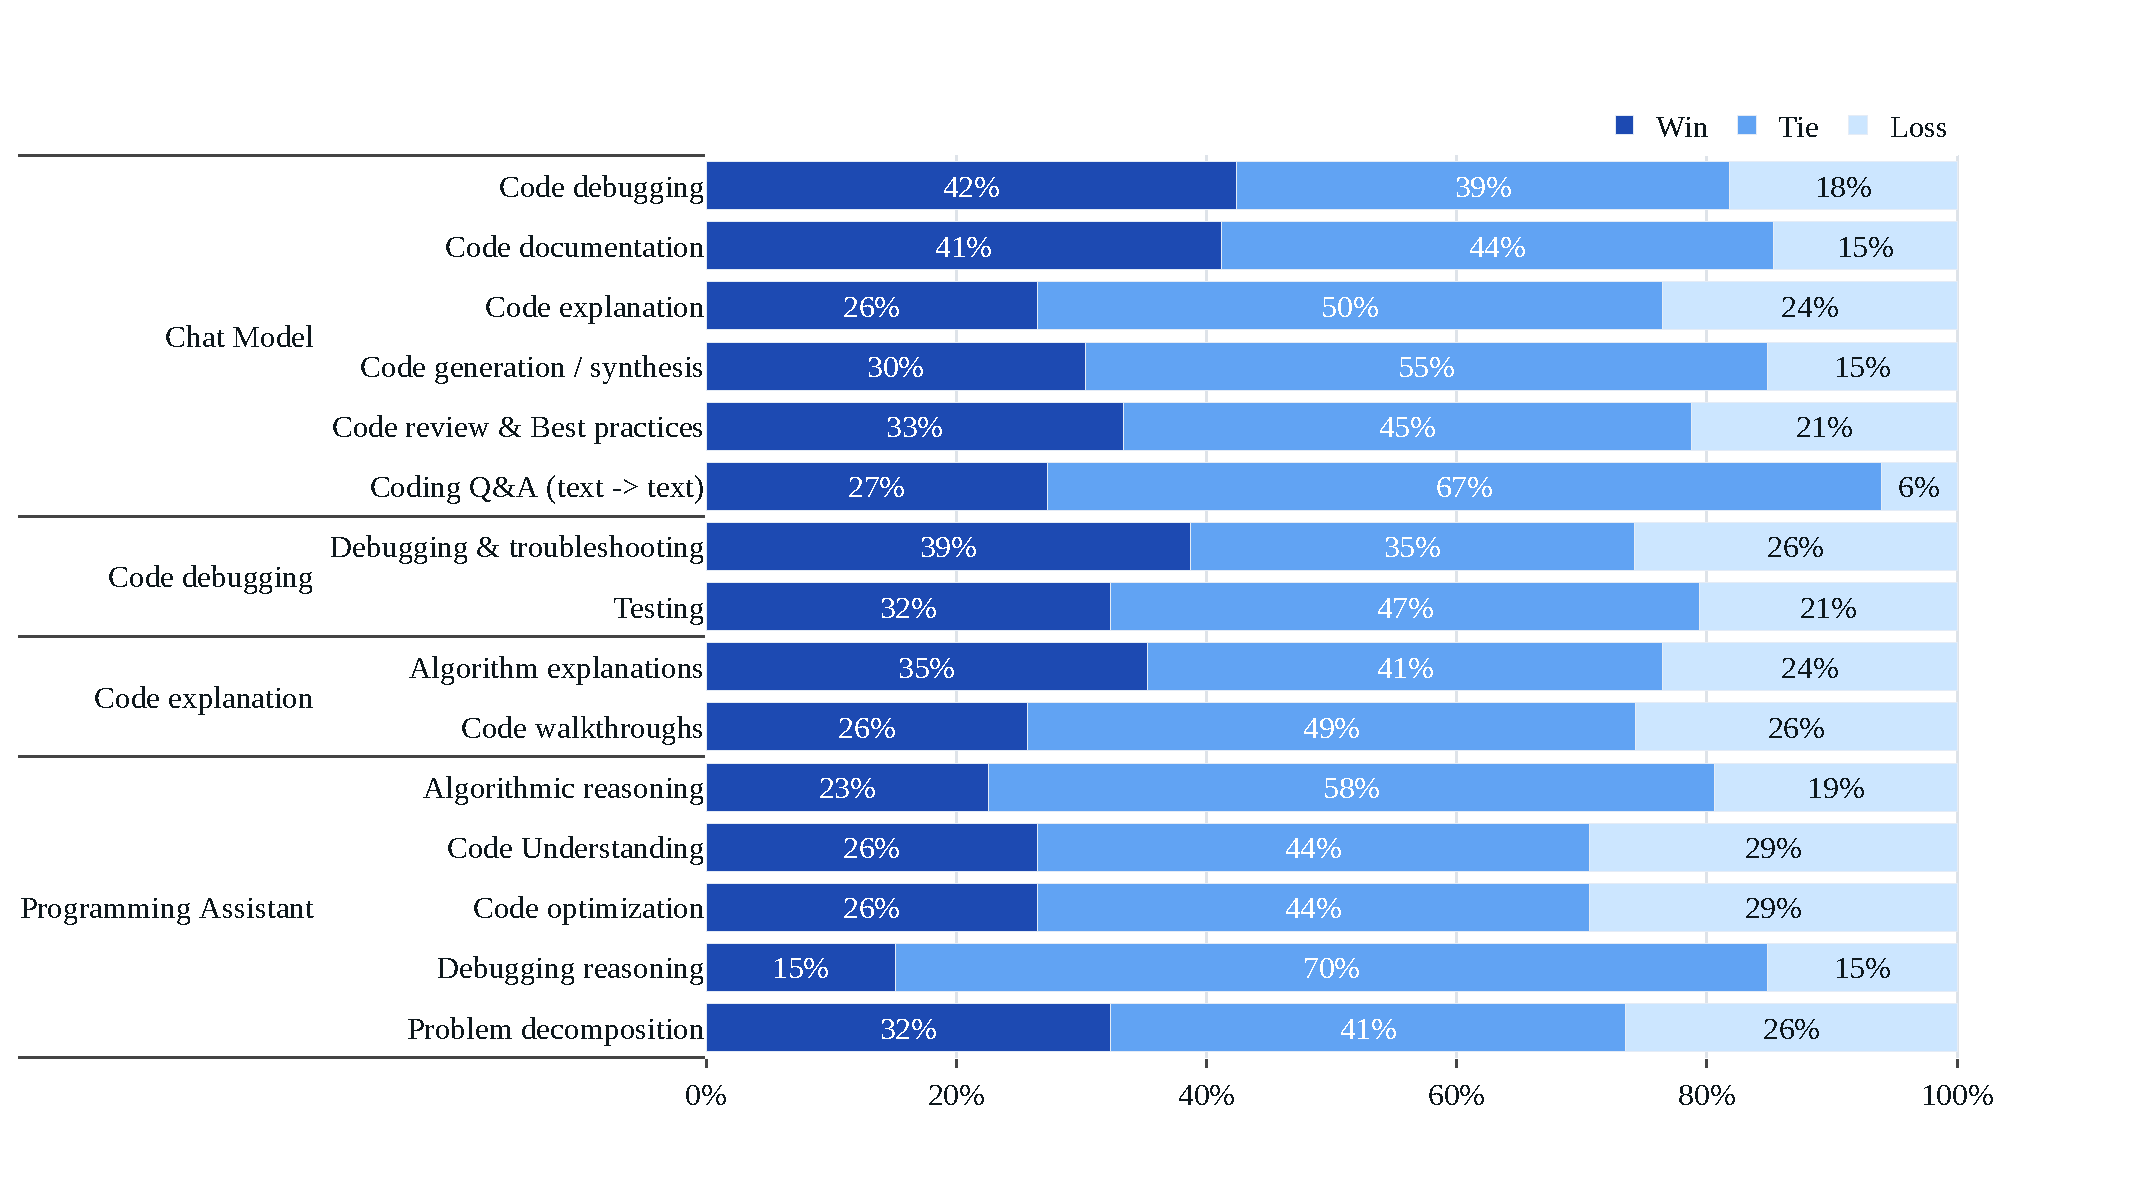
\includegraphics[width=0.75\linewidth]{assets/heval-gpt4preview-multiturn-coding-l2.pdf}
    \caption{Human evaluation results comparing the multiturn coding capability of Llama 3 405B vs. GPT-4 across subcategories.}
    \label{fig:heval-gpt4o-multiturn-coding-l2.png}
\end{figure}
